
\chapter{Requirements Analysis}


% 1) Introduction
% Section introducing the AgriGov Market platform
\section{Introduction}

While the strategic importance of digitalizing Algeria's agricultural sector is well-recognized, the transition from traditional, informal market structures to a transparent digital ecosystem requires a rigorous understanding of the field's functional needs. The current reliance on over-intermediation and asymmetric price information \cite{CIHEAM2025} creates a complex environment that the \textbf{AgriGov Market} platform aims to restructure. To build a system that effectively bridges the gap between farmers, transporters, and the Ministry of Agriculture, it is first necessary to conduct a thorough analysis of the requirements and the existing operational challenges.

The objective of this chapter is to lay the analytical foundation for the proposed system. By exploring the requirements from both a technical and a business perspective, we identify the specific boundaries of the system and define how various actors will interact within this new digital framework. This phase is crucial for ensuring that the final software solution is not only technically sound but also aligned with the strategic objectives of the Ministry of Agriculture.

The remainder of this chapter is organized as follows. First, we provide a detailed study of existing systems and their limitations to justify our proposed approach. We then proceed to identify the various actors involved and present a static context diagram to visualize the system's environment. Subsequently, we identify and model the core use cases, providing detailed textual specifications and system sequence diagrams for the most critical functionalities. The chapter also previews the primary human-machine interfaces before concluding with a synthesis of the requirements that will guide the design phase.

% 2) Étude de l’existant
%----------existing systems---------------------
\section{Existing Systems}
% ============================================================

In order to better understand existing digital solutions in agricultural trade, three representative digital platforms were analyzed.
The analyzed digital platforms take into account different approaches to digitalization in the agricultural trade market.

The purpose of this analysis is to identify its strengths and weaknesses in
order to properly position the proposed AgriGov Market platform:

% ============================================================
\subsection{Farmers Business Network (FBN) -- United States}

Farmers Business Network (FBN), which began operations in 2014 in the United States, is a private digital agricultural network that aims to improve price transparency and data sharing among farmers. The network, which has thousands of farmers across North America, offers price comparison services for farmers, direct selling options, agronomic information based on collective data, as well as financial services \cite{wolfert2017}.

\begin{figure}[H]
	\centering
	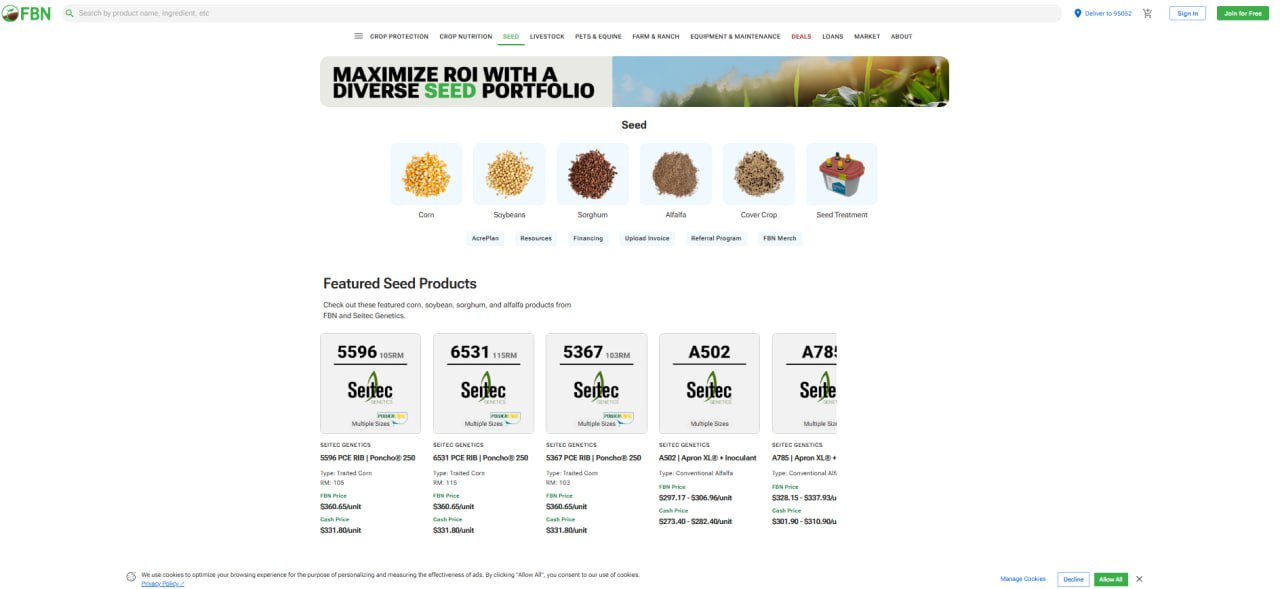
\includegraphics[width=0.8\textwidth]{images/existingHome/fbn_interface.png}
	\caption{FBN-Interface :https://www.fbn.com/}
	\label{fig:fbn}
\end{figure}

% ============================================================
\subsection{eNAM (Electronic National Agriculture Market) -- India}

Electronic National Agriculture Market (eNAM) is a government-driven project launched in 2016 to integrate Indian agricultural markets at a national level.
eNAM provides a link between Agricultural Produce Market Committees (APMCs) via an online trading system that allows nationwide bidding, quality assessment, and direct bank transfers for farmers.

As a government-driven project, eNAM is a remarkable institutional effort to promote and regulate agricultural trade.

\begin{figure}[H]
	\centering
	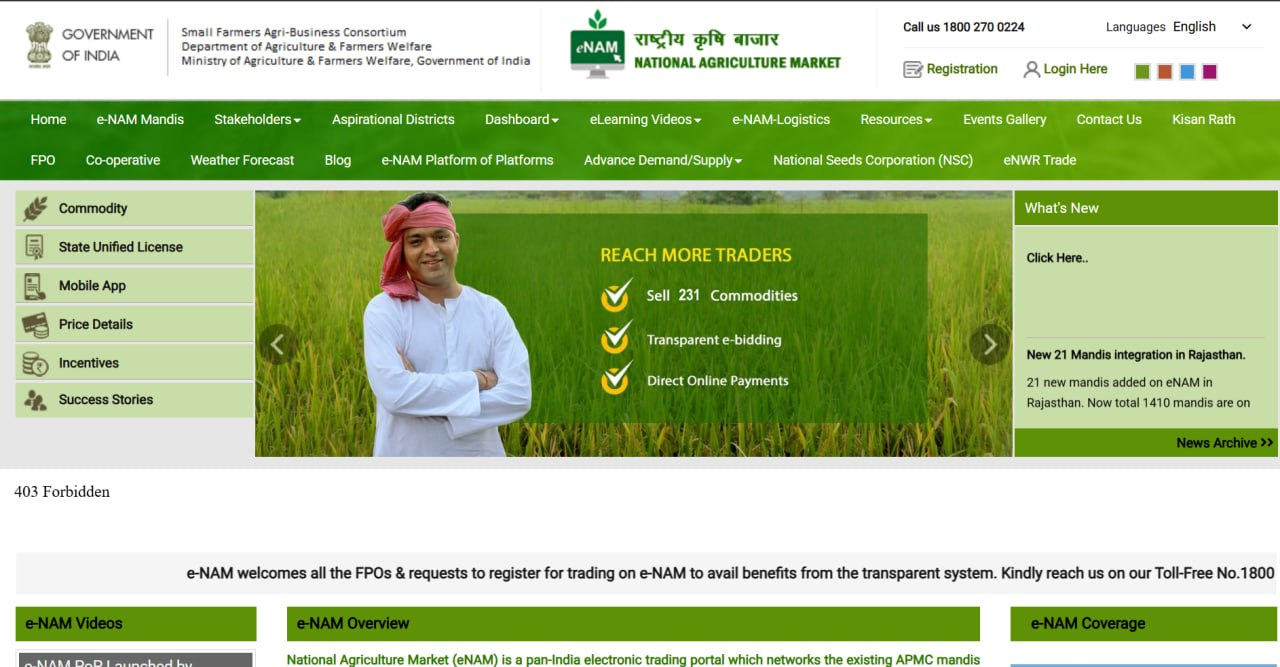
\includegraphics[width=0.8\textwidth]{images/existingHome/enam_interface.png}
	\caption{eNAM :www.enam.gov.in}
	\label{fig:enam}
\end{figure}

% ============================================================
% ============================================================
\subsection{Ghana Agriculture and Agribusiness Platform (GhAAP) -- Ghana}

The Ghana Agriculture and Agribusiness Platform (GhAAP) is a web-based platform developed in Ghana to support farmers and agribusiness actors through multiple digital services. The platform allows users to request farm services such as mechanization, spraying, and harvesting operations. 

It also connects farmers with agricultural extension agents who provide professional advice and technical support. In addition, the platform enables farmers to list and sell their agricultural products directly, while linking users to other commodity trading platforms to expand market access.

Through real-time information sharing, GhAAP improves coordination, transparency, and monitoring across the agricultural value chain.

\begin{figure}[H]
	\centering
	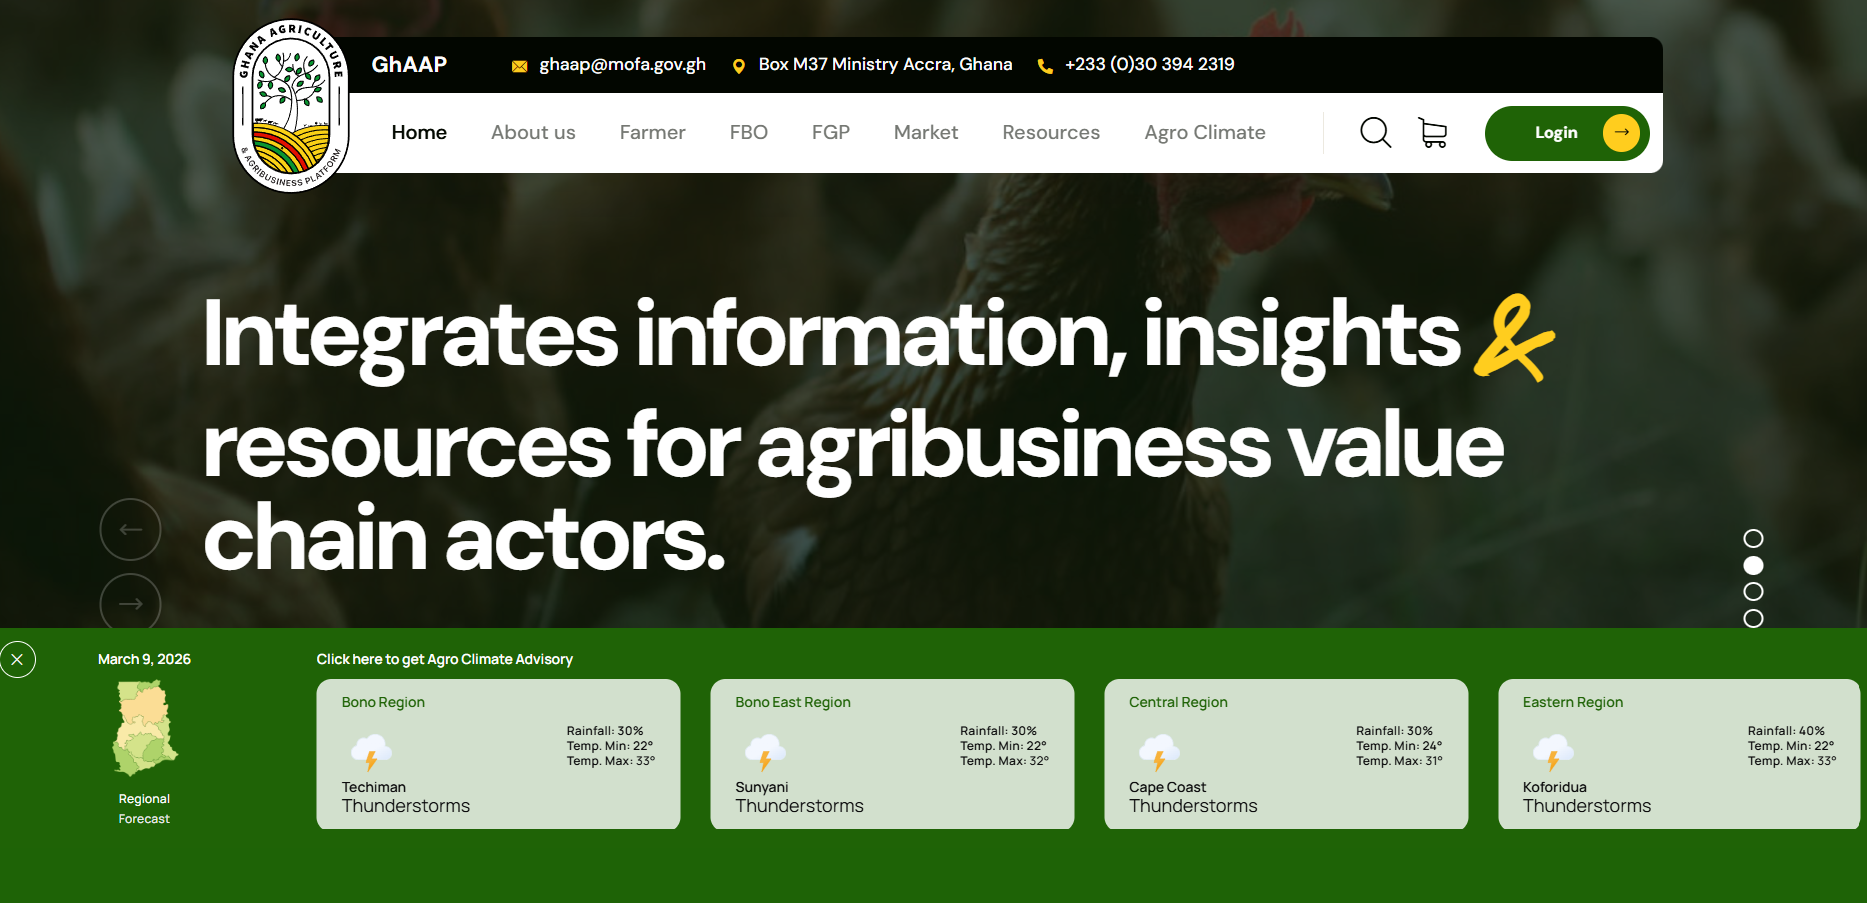
\includegraphics[width=0.8\textwidth]{images/existingHome/ghaap_interface.png}
	\caption{GhAAP: https://ghaap.com/}
	\label{fig:ghaap}
\end{figure}

% ============================================================

\subsection{Limitations and our solutions}
\begin{table}[H]
	\centering
	\begin{tabular}{|p{2.5cm}|p{2cm}|p{4.5cm}|p{4cm}|}
		\hline
		\textbf{System} & \textbf{Country} & \textbf{Strengths} & \textbf{Limitations} \\
		\hline
		FBN & USA & Price transparency, collaborative network, agronomic analytics & Paid model, no logistics integration, no government supervision \\
		\hline
		eNAM & India & Government-backed, national integration, quality testing, logistics module & Infrastructure gaps, digital divide, regulatory complexity \\
		\hline
		Ghana Agriculture and Agribusiness Platform (GhAAP) & Ghana & Farm services, extension advice, direct selling, links to other markets & National platform only, limited information on pricing mechanisms \\
		\hline
	\end{tabular}
	\caption{Comparative Analysis of Existing Systems}
	\label{tab:existing-systems}
\end{table}

Although Table \ref{tab:existing-systems} highlights the main characteristics of each platform, a deeper comparative analysis reveals important insights.

First, the studied systems adopt different operational models. FBN represents a \textbf{private and data-driven approach}, focusing on price transparency and analytics, but lacking institutional regulation. In contrast, eNAM follows a \textbf{government-driven model}, ensuring market integration and regulatory oversight, although it faces challenges related to infrastructure and system complexity. GhAAP, on the other hand, adopts a \textbf{service-oriented approach}, combining advisory services and market access, but remains limited in terms of scalability and pricing transparency.

Second, none of these platforms provides a \textbf{fully integrated solution}. While FBN lacks logistics and governance, eNAM struggles with accessibility and implementation constraints, and GhAAP does not offer advanced pricing mechanisms or national-level coordination.

These observations highlight a critical gap: the absence of a unified platform that combines \textbf{market transparency, logistics management, and governmental supervision} within a single system.

Therefore, AgriGov Market aims to address these limitations by proposing an integrated and institutional solution adapted to the Algerian context, ensuring better coordination between actors, improved price regulation, and enhanced transparency across the agricultural value chain.

% ============================================================
\subsubsection{Discussion}

In this context, AgriGov Market is positioned as an institutional and integrated digital platform tailored to Algeria. It combines product commercialization, logistics coordination, and regulatory supervision under the authority of the Ministry of Agriculture, aiming to ensure transparency, market stability, and modernization of the national agricultural value chain.






% 3) Acteurs + contexte statique

% Identification of Actors and Their Roles
\section{Identification of Actors and Static Context Diagram}
% ==================================================

In order to define the system boundaries and understand the system's operation environment, it is necessary to define the different actors that interact with the AgriGov Market system. These actors represent the external world in our system: 


%------------------------------------------
\subsection{Farmer}

Farmers are agricultural producers who cultivate and supply agricultural products through the AgriGov platform.

\begin{itemize}
	\item Grow and provide fresh fruits and vegetables to the markets.
	\item Commercialization of agricultural production in an efficient manner.
	\item Management of agricultural farms by keeping product availability updated.
	\item Confirm or reject orders.
	\item Control of sales and revenue to make business decisions.
\end{itemize}

%------------------------------------------
\subsection{Buyer}

Buyers are individuals or organizations (retailers, wholesalers, restaurants, or end consumers) who purchase agricultural products via the platform.

\begin{itemize}
	\item Buyers include individual buyers, retailers and wholesalers looking for fresh products.
	\item Transparent purchase of products.
	\item Browse and search products on the platform.
	\item Tracking the delivery of products.
	\item Establishing long-term relationships with farmers.
	\item Moving from intermediaries to direct connection with farmers.
\end{itemize}

%------------------------------------------
\subsection{Transporter}

Transporters are logistics operators responsible for delivering agricultural products from farmers to buyers.

\begin{itemize}
	\item Carry products from farms to buyers.
	\item Viewing available delivery opportunities.
	\item Selection of delivery missions along their routes.
	\item Collection of products from farms.
	\item Providing status updates during transportation.
	\item Real-time tracking of farms.
\end{itemize}

%------------------------------------------
\subsection{Ministry}

The Ministry of Agriculture is the official governmental authority and owner of the AgriGov platform.

\begin{itemize}
	\item Oversees the food system.
	\item Establishment of rules ensuring fairness and transparency.
	\item Control of participation in the food system through approval and validation of farmers, buyers, and transporters.
	\item Definition of product categories used in the platform.
	\item Establishment of price references to prevent exploitation.
	\item Monitoring of production, distribution, and pricing of agricultural products.
	\item Support for shaping national agricultural policy.
	\item Protection of farmers and consumers through platform supervision.
\end{itemize}

%------------------------------------------
\subsection{Quality Inspector}

The Quality Inspector operates under the supervision of the Ministry of Agriculture and verifies product compliance.

\begin{itemize}
	\item Inspection of farms and collection points.
	\item Verification of product quality.
	\item Checking freshness, size, safety, and labeling of products.
	\item Comparison with government standards.
	\item Approval of products for listing when standards are met.
	\item Rejection of products that do not meet required standards.
	\item Protection of consumers from fraud.
	\item Assurance of fair competition among farmers.
\end{itemize}

%------------------------------------------
\subsection{Delivery Manager}

The Delivery Manager supervises and coordinates delivery operations.

\begin{itemize}
	\item Management of logistics operations.
	\item Assignment of delivery missions to transporters.
	\item Intervention in case of delivery problems or delays.
	\item Ensuring efficient product delivery.
	\item Minimization of delivery time and cost.
\end{itemize}

%------------------------------------------
\subsection{Payment System}

The Payment System is an external financial service integrated into the platform.

\begin{itemize}
	\item Facilitation of secure money transfer from buyer to farmer.
	\item Processing payments when orders are made.
	\item Verification of funds availability.
	\item Notification of users about transaction status.
	\item Protection of financial information through encryption.
	\item Support for digital trade operations.
\end{itemize}

%------------------------------------------
\subsection{Weather System}

The Weather System is an external service providing meteorological data.

\begin{itemize}
	\item Provide real-time weather forecasts.
	\item Support farmers in harvest and planting decisions.
	\item Assist transporters in avoiding weather-related delays.
	\item Alert users to extreme conditions (storms, frost, heatwaves).
	\item Enable better coordination of delivery schedules based on climate conditions.
\end{itemize}
%----------
\subsection{System Context Diagram}
\addcontentsline{toc}{section}{System Context Diagram}


According to Dennis et al. \cite{dennis2015}, a context diagram is a high-level graphical representation of a system that illustrates the system as a single process and defines its interactions with external entities. It establishes the system boundary and shows the flow of information between the system and its environment without revealing internal system processes. This type of diagram helps stakeholders understand the overall scope, external interfaces, and operational environment of the system.

\begin{figure}[H]
	\centering
	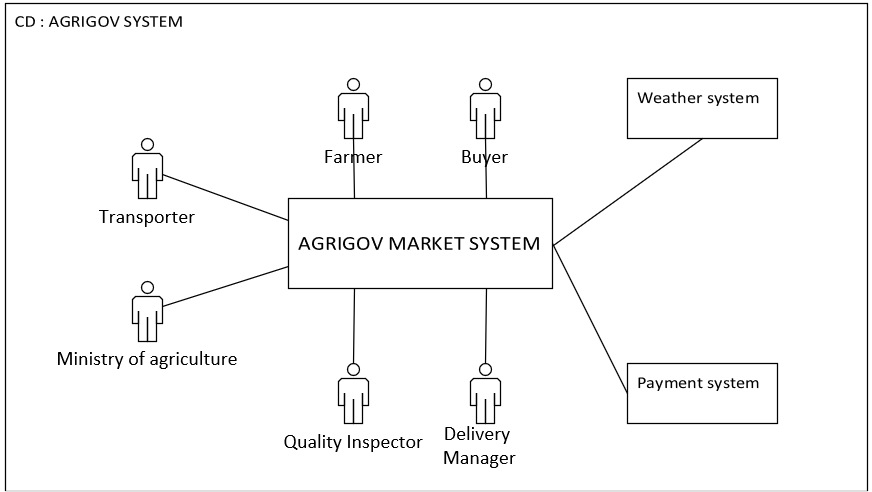
\includegraphics[width=1\textwidth]{images/diagrammes/DCS}
	\caption{AgriGov Market System Context Diagram}
	\label{fig:dcs}
\end{figure}

This diagram provides a global view of the system and helps identify all external actors and their interactions with the AgriGov Market platform. It serves as a foundation for further system analysis and design phases.

% 4) Cas d’utilisation
% ==================================================
% 4. Use Cases
% ==================================================
\section{Use Cases}

% --------------------------------------------------
% 4.1 Identification of Use Cases by Actor
% --------------------------------------------------

Based on the system analysis, the main use cases for each actor are summarized below. These use cases represent high-level functional interactions with the AgriGov Market platform.

% =========================
% Buyer
% =========================
\subsection{Buyer}

The buyer is considered the end user of the platform so he will have the ability to search through the available products offered by the farmers, which will be helpful for them to purchase the required products. They will be able to place new orders or cancel their existing ones. In addition, they will have the ability to monitor their deliveries and their previous purchase history. Once they receive their ordered products, they will have the ability to provide feedback and evaluations, which will be helpful to improve the quality of the products and increase trust between buyers and farmers.

\begin{figure}[H]
	\centering
	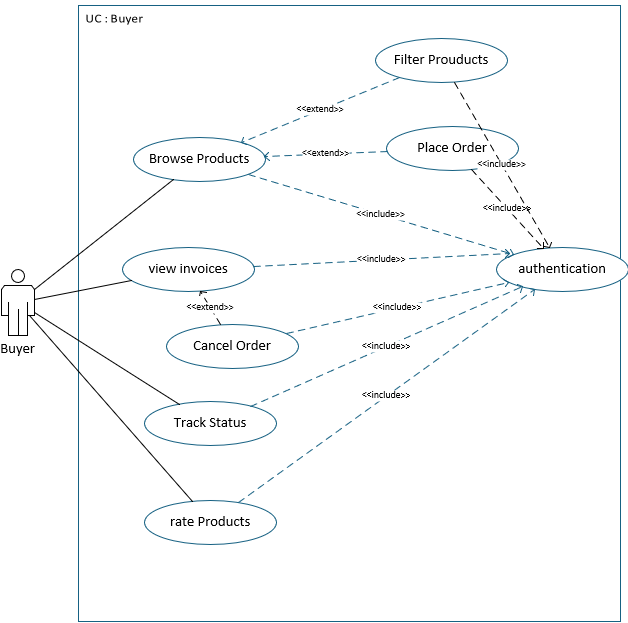
\includegraphics[width=0.95\textwidth]{images/diagrammes/buyerUCD}
	\caption{Use Case Diagram -- Buyer}
	\label{fig:buyer_ucd}
\end{figure}


% =========================
% Farmer
% =========================
\subsection{Farmer}

The farmer is  responsible for providing the agricultural products on  the platform. he has the ability to manage information of the farm and the products being offered, Moreover, the farmer has the responsibility of managing orders from customers, including processing purchase requests while keeping track of the status of each purchase order and update that status. The farmer also has access to information regarding market prices, enabling them to keep track of the latest trends in the agricultural market. Finally, the farmer has the responsibility of coordinating transportation requests, ensuring that products are transported to customers.


\begin{figure}[H]
	\centering
	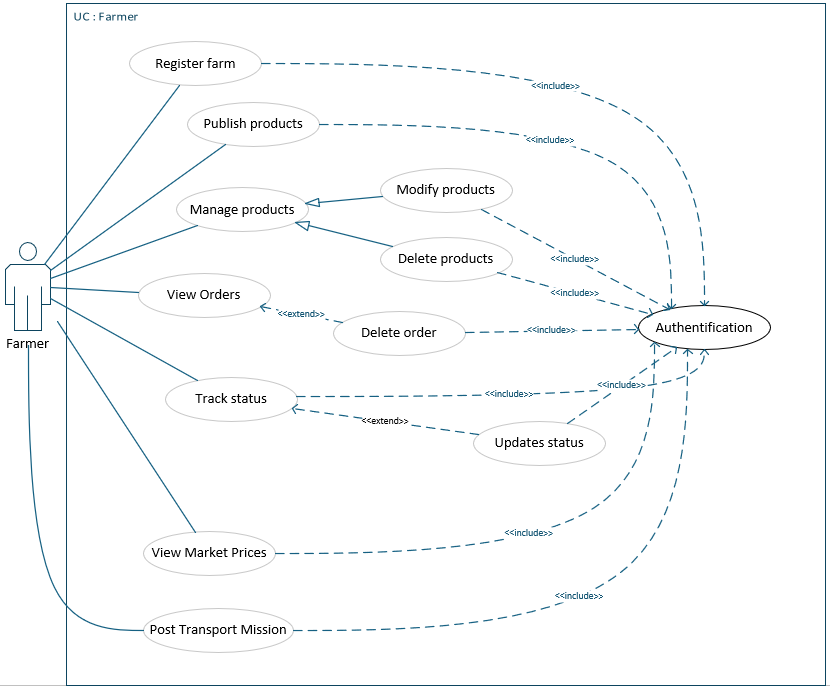
\includegraphics[width=1.05\textwidth]{images/diagrammes/farmerUCD}
	\caption{Use Case Diagram -- Farmer}
	\label{fig:farmer_ucd}
\end{figure}



% =========================
% Transporter
% =========================
\subsection{Transporter}

The function of the transporter is to handle the logistics in the delivery of the agricultural products to the buyers. Transporters are responsible for managing their transportation availability in the system, which allows them to indicate when they are available to handle the delivery request. The transporters are able to accept or reject the delivery requests submitted to transport the products. After that, the transporters are responsible for executing the delivery mission by transporting the products to the farmer or the destination. During the execution of the delivery mission, the transporters are responsible for managing the delivery status to ensure transparency in the process.


\begin{figure}[H]
	\centering
	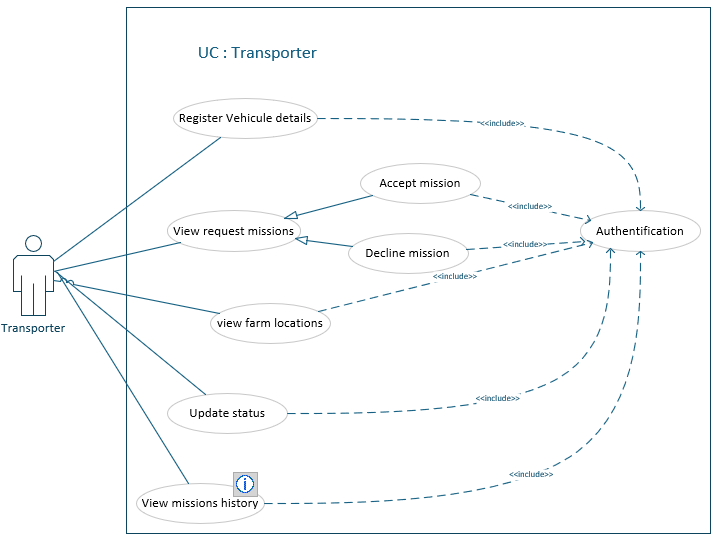
\includegraphics[width=1.05\textwidth]{images/diagrammes/transporterUCD}
	\caption{Use Case Diagram -- Transporter}
	\label{fig:transporter_ucd}
\end{figure}


% =========================
% Ministry (Administrator)
% =========================
\subsection{Ministry (Administrator)}

The ministry oversees and regulates the official information provided within the platform to ensure that the system is well governed and efficient. The ministry is also responsible for the management of the validation of the users and the regulation of access to the system, ensuring that the users are properly authorized, for instance, the farmers, the buyers, and the transporters. The ministry is also responsible for regulating the various products and the official prices within the market to ensure that there is transparency and fairness within the agricultural market. The ministry is also responsible for overseeing the overall operations within the system, including the activities within the market, to ensure that the activities within the system are in conformity with the regulations and standards.

\begin{figure}[H]
	\centering
	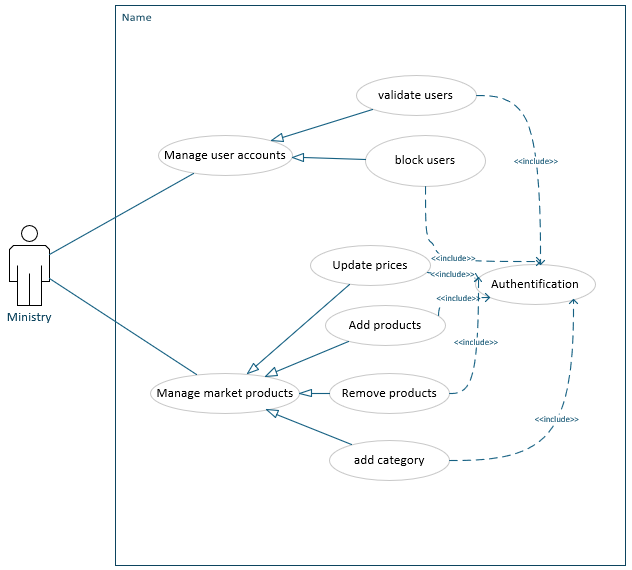
\includegraphics[width=0.95\textwidth]{images/diagrammes/ministryUCD}
	\caption{Use Case Diagram -- Ministry (Administrator)}
	\label{fig:ministry_ucd}
\end{figure}
we resume the use-cases in the globaleUCD below :
%----------global-UC------
\begin{figure}[H]
	\centering
	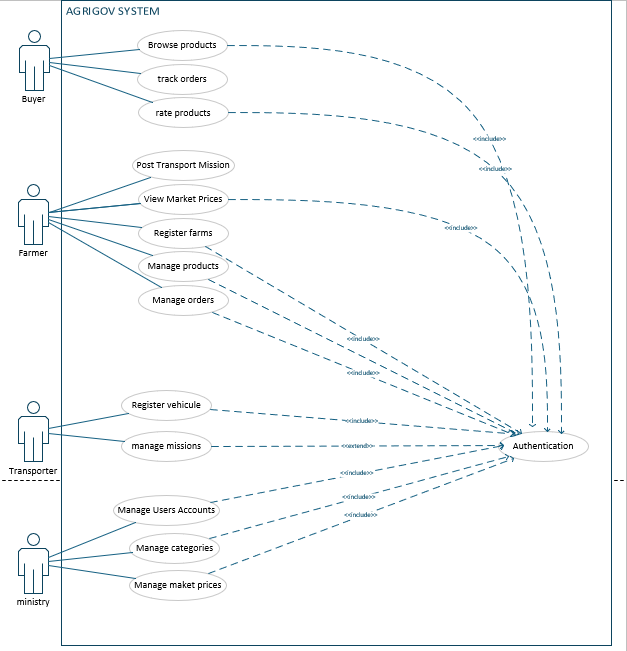
\includegraphics[width=1.15\textwidth]{images/diagrammes/GlobalUCD}
	\caption{Use Case Diagram -- Globale}
	\label{fig:Global_UC}
\end{figure}

% 5) Spécification des cas principaux
% ==================================================
% Main Use Cases Description
% ==================================================
\section{Description of the Main Use Cases}

This section provides a detailed description of the main use cases of the proposed system. Each use case is presented through its actors, preconditions, nominal flow, as well as alternative and exceptional scenarios. In addition, system sequence diagrams are provided to illustrate the dynamic interactions between the user and the system.

% ==================================================
% UC01 -- Authentication
% ==================================================

\subsection{UC01 -- User Authentication (Login)}

\begin{table}[H]
	\centering
	\renewcommand{\arraystretch}{1.3}
	\begin{tabular}{|p{4cm}|p{10cm}|}
		\hline
		
		\textbf{Use Case Name} & Authentication \\ 
		\hline
		
		\textbf{Primary Actor} & User\\ 
		\hline
		
		\textbf{Preconditions} &
		\begin{itemize}
			\item The user has a valid account.
		\end{itemize} \\ 
		\hline
		
		\textbf{Nominal Sequence} &
		\begin{enumerate}
			\item The user accesses the login page.
			\item The system displays the authentication form.
			\item The user enters credentials and submits the form.
			\item The system validates the credentials.
			\item The system grants access and creates a session.
		\end{enumerate} \\ 
		\hline
		
		\textbf{Alternative Sequence} &
		\textbf{A1 -- Invalid input format}
		\begin{itemize}
			\item The system detects missing or incorrect data.
			\item The user is asked to correct the input.
		\end{itemize} \\ 
		\hline
		
		\textbf{Exceptional Sequence} &
		\textbf{E1 -- Incorrect credentials}
		\begin{itemize}
			\item The system declines authentication.
			\item An error message is displayed.
		\end{itemize} \\ 
		\hline
		
		\textbf{Postcondition} &
		The user is authenticated and redirected to the appropriate dashboard. \\ 
		\hline
		
	\end{tabular}
	\caption{Use Case Description -- User Authentication}
\end{table}

\begin{figure}[H]
	\hspace{-1.5cm}
	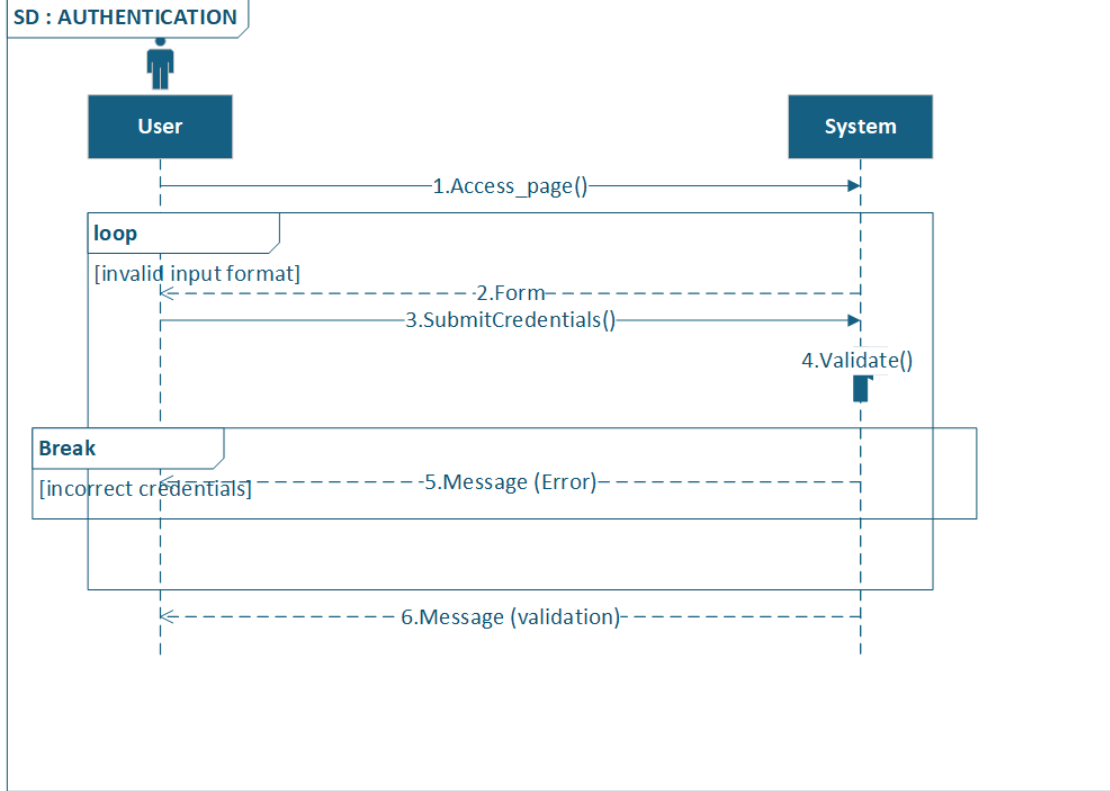
\includegraphics[width=1.15\textwidth]{images/diagrammes/Authentication}
	\caption{System Sequence Diagram -- UC01 Authentication}
\end{figure}


This diagram illustrates the interaction between the user and the system during the authentication process. The user initiates the process by entering credentials. The system then validates the provided information and responds either by granting access (successful authentication) or by displaying an error message in case of failure.

% ==================================================
% UC02
% ==================================================

\subsection{UC02 -- Decide Delivery Mission}

\begin{table}[H]
	\centering
	\renewcommand{\arraystretch}{1.3}
	\begin{tabular}{|p{4cm}|p{10cm}|}
		\hline
		
		\textbf{Use Case Name} & Decide Delivery Mission \\ 
		\hline
		
		\textbf{Primary Actor} & Transporter \\ 
		\hline
		
		\textbf{Objective} & Accept or reject a delivery mission. \\ 
		\hline
		
		\textbf{Preconditions} &
		\begin{itemize}
			\item The transporter is authenticated.
			\item A delivery request exists.
		\end{itemize} \\ 
		\hline
		
		\textbf{Nominal Sequence} &
		\begin{enumerate}
			\item The system sends a delivery request.
			\item The transporter views mission details.
			\item The transporter accepts the mission.
			\item The system records and updates the mission.
		\end{enumerate} \\ 
		\hline
		
		\textbf{Alternative Sequence} &
		\textbf{A1 -- Mission Rejected}
		\begin{itemize}
			\item The transporter rejects the mission.
			\item The system searches for another transporter.
		\end{itemize} \\ 
		\hline
		
		\textbf{Exceptional Sequence} & 
		\textbf{E1 -- No Transporter Available in Region}
		\begin{itemize}
			\item The system fails to find an available transporter within the specified geographical region.
			\item The system flags the mission status as pending.
		\end{itemize} \\ 
		\hline
		
		\textbf{Postcondition} &
		The mission is assigned if accepted. \\ 
		\hline
		
	\end{tabular}
	\caption{Use Case Description -- Decide Delivery Mission}
\end{table}

\begin{figure}[H]
	\hspace{-1.5cm}
	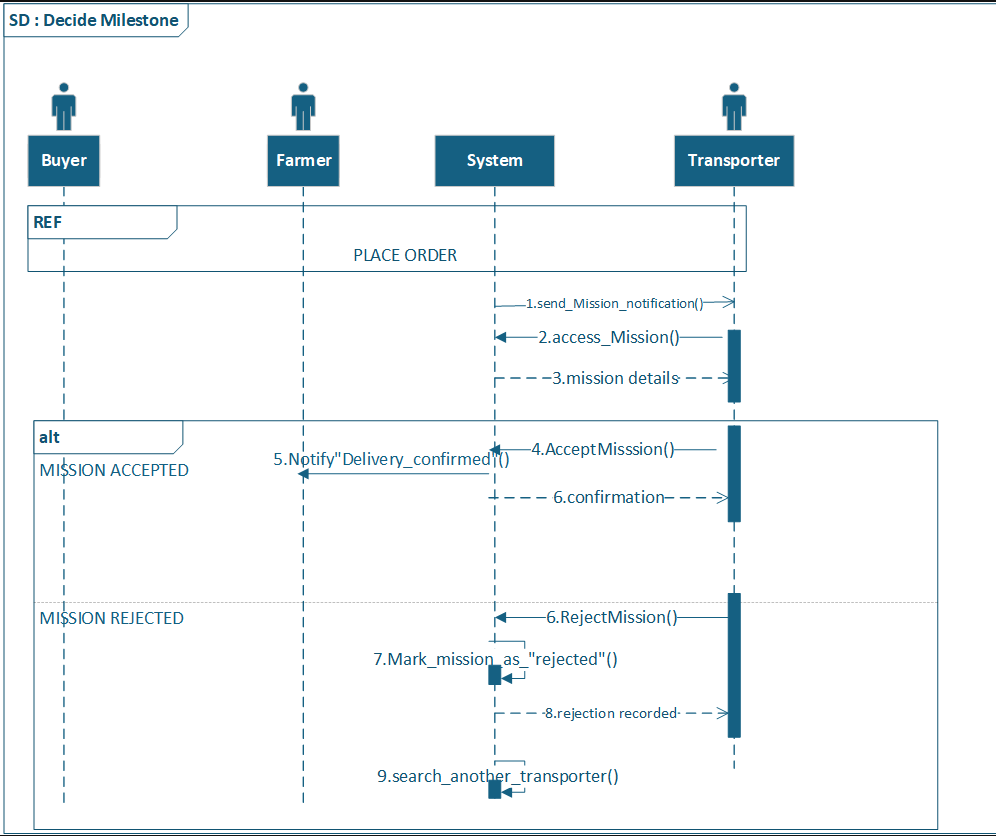
\includegraphics[width=1.15\textwidth]{images/diagrammes/DecideMilestone}
	\caption{System Sequence Diagram -- Decide Delivery Mission}
\end{figure}

 
This diagram shows how the system interacts with the transporter when a delivery request is issued. The system sends a notification, and the transporter evaluates the mission details before making a decision. Based on this decision, the system updates the mission status and notifies the relevant actors.

% ==================================================
% UC03
% ==================================================

\subsection{UC03 -- User Validation}

\begin{table}[H]
	\centering
	\renewcommand{\arraystretch}{1.3}
	\begin{tabular}{|p{4cm}|p{10cm}|}
		\hline
		
		\textbf{Use Case Name} & User Validation \\ 
		\hline
		
		\textbf{Primary Actor} & Ministry Administrator \\ 
		\hline
		
		\textbf{Objective} & Approve or reject user registration. \\ 
		\hline
		
		\textbf{Preconditions} & Authentication \\ 
		\hline
		
		\textbf{Nominal Sequence} &
		\begin{enumerate}
			\item The user submits a registration request.
			\item The system stores the request.
			\item The administrator reviews the information.
			\item The administrator approves the request.
			\item The system notifies the user.
		\end{enumerate} \\ 
		\hline
		
		\textbf{Alternative Sequence} & 
		\textbf{A1 -- Documents Unclear}
		\begin{itemize}
			
			\item The system requests the user to re-submit clearer information or higher-quality documents.
			\item The registration request remains in a pending status until the user updates it.
		\end{itemize} \\ 
		\hline
		
		\textbf{Exceptional Sequence} &
		\textbf{E1 -- Invalid documents}
		\begin{itemize}
			\item The request is rejected.
			\item The user is notified.
		\end{itemize} \\ 
		\hline
		
		\textbf{Postcondition} &
		The account is activated. \\ 
		\hline
		
	\end{tabular}
	\caption{Use Case Description -- User Validation}
\end{table}

\begin{figure}[H]
	\hspace{-1.5cm}
	\includegraphics[width=1.15\textwidth]{images/diagrammes/userValidation}
	\caption{System Sequence Diagram -- User Validation}
\end{figure}

 
This diagram represents the validation process handled by the administrator. After a registration request is submitted, the system stores it and allows the administrator to review it. The final decision (approval or rejection) is then communicated to the user.

% ==================================================
% UC04
% ==================================================

\subsection{UC04 -- Search Product}

\begin{table}[H]
	\centering
	\renewcommand{\arraystretch}{1.3}
	\begin{tabular}{|p{4cm}|p{10cm}|}
		\hline
		
		\textbf{Use Case Name} & Search Product \\ 
		\hline
		
		\textbf{Primary Actor} & Buyer \\ 
		\hline
		
		\textbf{Objective} & Search for available products. \\ 
		\hline
		
		\textbf{Preconditions} & \begin{itemize}
			\item The user is authenticated.
		\end{itemize}  \\ 
		\hline
		
		\textbf{Nominal Sequence} &
		\begin{enumerate}
			\item The user enters a keyword in the search bar.
			\item The system processes the request.
			\item The system displays matching products.
		\end{enumerate} \\ 
		\hline
		
		\textbf{Alternative Sequence} & 
		\textbf{A1 -- Filtered Search}
		\begin{itemize}
			\item The user applies specific search filters (e.g., category, price range, region, or availability).
			\item The system refines the search query based on the selected parameters.
			\item The system displays the filtered list of products matching the criteria.
		\end{itemize} \\ 
		\hline
		
		\textbf{Exceptional Sequence} &
		\textbf{E1 -- No results found}
		\begin{itemize}
			\item The system displays a "No products match your search" message.
			\item The system suggests alternative keywords or prompts the user to clear applied filters.
		\end{itemize} \\ 
		\hline
		
		\textbf{Postcondition} &
		A list of products matching the user's search or filter criteria is displayed. \\ 
		\hline
		
	\end{tabular}
	\caption{Use Case Description -- Search Product}
\end{table}

\begin{figure}[H]
	\centering
	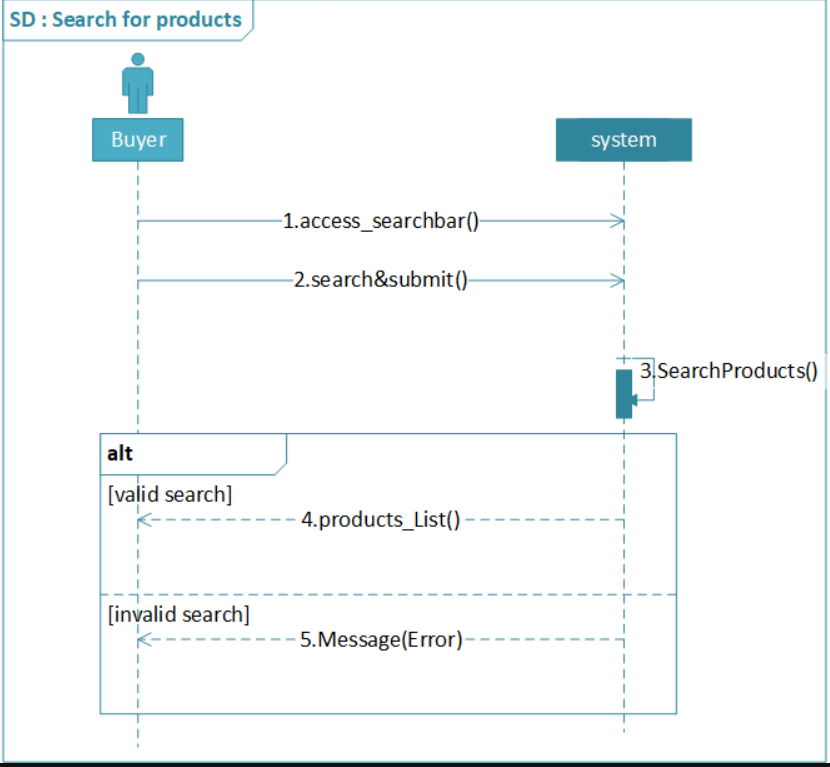
\includegraphics[width=0.95\textwidth]{images/diagrammes/SearchProduct}
	\caption{System Sequence Diagram -- Search Product}
\end{figure}

This diagram illustrates how the buyer interacts with the system to search for products. The user submits a query, and the system processes it to retrieve and display relevant results. If no products match the query, an appropriate message is returned.

% ==================================================
% UC05
% ==================================================

\subsection{UC05 -- Decide Order}

\begin{table}[H]
	\centering
	\renewcommand{\arraystretch}{1.3}
	\begin{tabular}{|p{4cm}|p{10cm}|}
		\hline
		
		\textbf{Use Case Name} & Decide Order \\ 
		\hline
		
		\textbf{Primary Actor} & Farmer \\ 
		\hline
		
		\textbf{Objective} & Accept or refuse an order. \\ 
		\hline
		
		\textbf{Preconditions} & The farmer is authenticated \\ 
		\hline
		
		\textbf{Nominal Sequence} &
		\begin{enumerate}
			\item The farmer views pending orders.
			\item The farmer selects an order.
			\item The farmer accepts the order.
			\item The system updates the status.
		\end{enumerate} \\ 
		\hline
		
		\textbf{Alternative Sequence} &
		\textbf{A1 -- Order Refused}
		\begin{itemize}
			\item The farmer refuses the order.
			\item The system updates the status.
		\end{itemize} \\ 
		\hline
		
		\textbf{Exceptional Sequence} & 
		\textbf{E1 -- No Pending Orders Found}
		\begin{itemize}
			
			\item The system displays an empty state message (e.g., "No pending orders available") and the use case terminates.
		\end{itemize} \\ 
		\hline
		
		\textbf{Postcondition} &
		The order status is updated. \\ 
		\hline
		
	\end{tabular}
	\caption{Use Case Description -- Decide Order}
\end{table}

\begin{figure}[H]
	\centering
	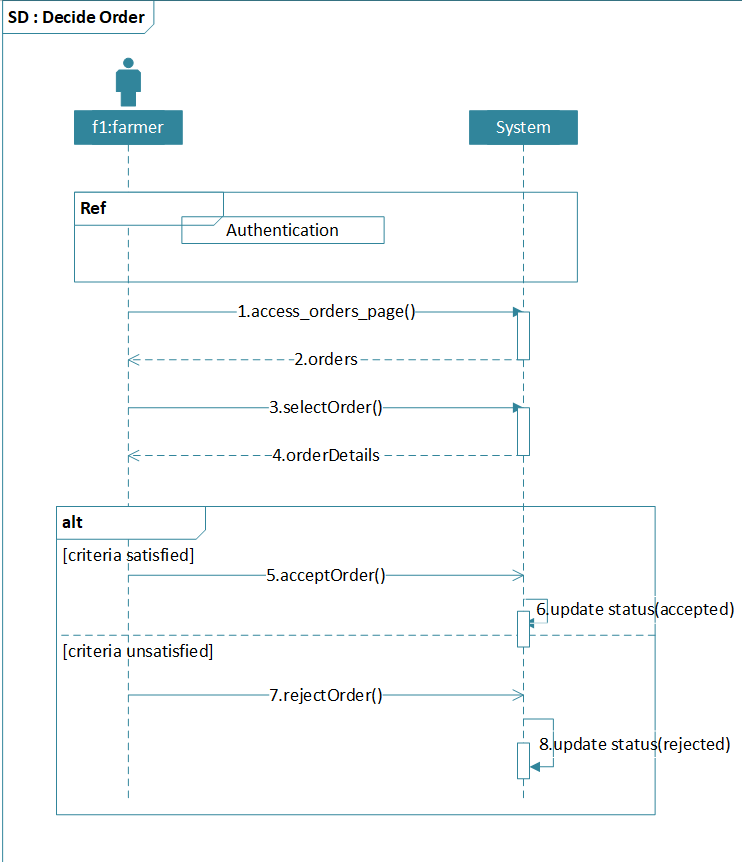
\includegraphics[width=0.95\textwidth]{images/diagrammes/decideOrder}
	\caption{System Sequence Diagram -- Decide Order}
\end{figure}

This diagram shows the interaction between the farmer and the system when handling orders. The farmer reviews order details and makes a decision. The system then records this decision and updates the order status accordingly.

% 6) IHM
%====================================================
% User Interface Mockups
%====================================================
\section{User Interface Mockups}
\label{sec:mockups}

Mockups represent the visual design and layout of the AgriGov Market system interfaces. 
They illustrate how users interact with the system and provide a clear vision of the system’s graphical structure before implementation.

These mockups were designed to ensure usability, efficiency, and accessibility for all actors of the platform.


\subsection{global Interface Structure}
According to \cite{pressman2014}, navigation diagrams are used in user interface design to model the interaction flow between screens and to ensure that users can efficiently access system functionalities. They help designers and stakeholders understand how information and actions are organized within the interface.

In the context of the AgriGov Market platform, navigation diagrams are used to represent the navigation paths available to each actor (farmer, buyer, transporter, and administrator), showing how users access the different services provided by the system.
\begin{figure}[H]
	\hspace{-2.2cm} % adjust this value
	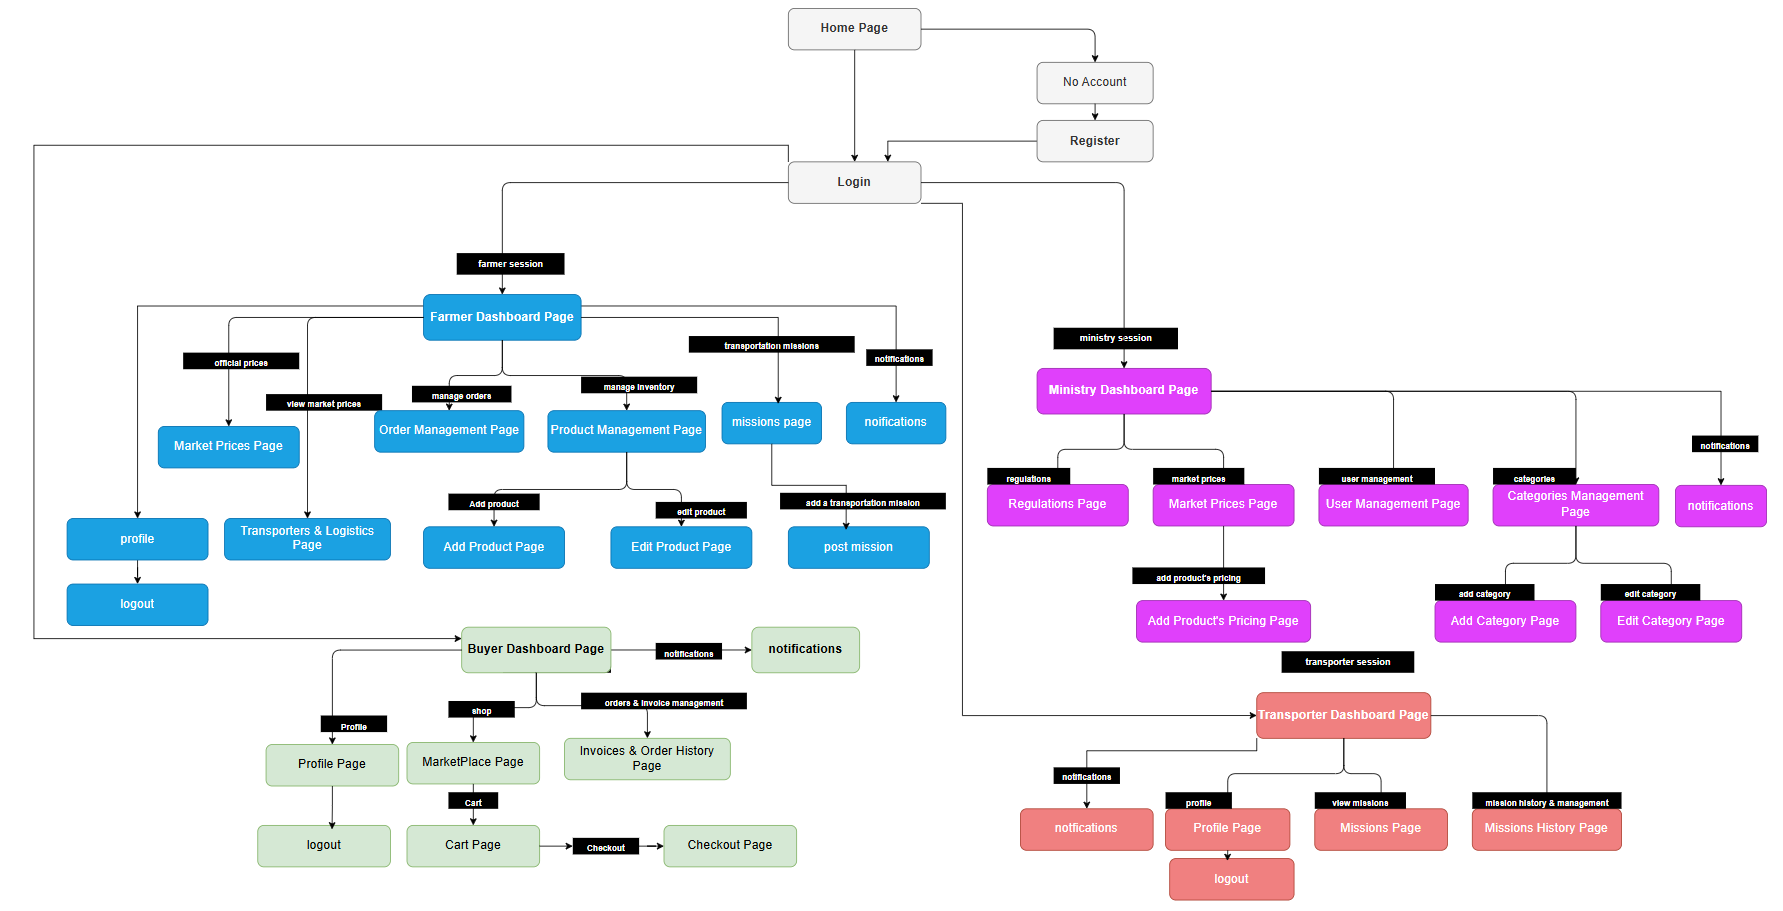
\includegraphics[width=1.3\textwidth]{images/navigation/global-navigation}
	\caption{Global Navigation Diagram}
	\label{fig:global-navigation}
\end{figure}

%----------------------------------------------------
\subsection{Farmer Interface}

A navigation diagram represents the structure and flow of navigation between the different user interfaces of a system. It illustrates how users move from one screen to another and highlights the relationships between the various pages or functionalities of the application. 


\begin{figure}[H]
	\centering
	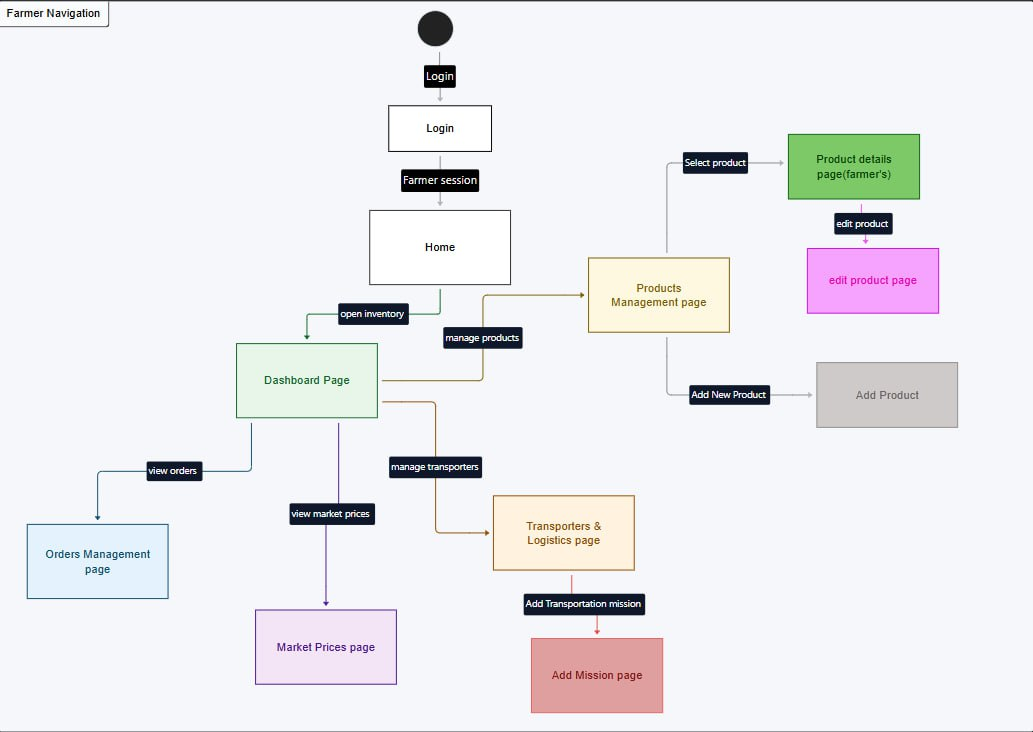
\includegraphics[width=0.9\textwidth]{images/navigation/farmer-navigation}
	\caption{Farmer Navigation Diagram}
	\label{fig:farmer-navigation}
\end{figure}
\begin{figure}[H]
	\centering

% Row 1
\begin{subfigure}[b]{0.45\textwidth}
	\centering
	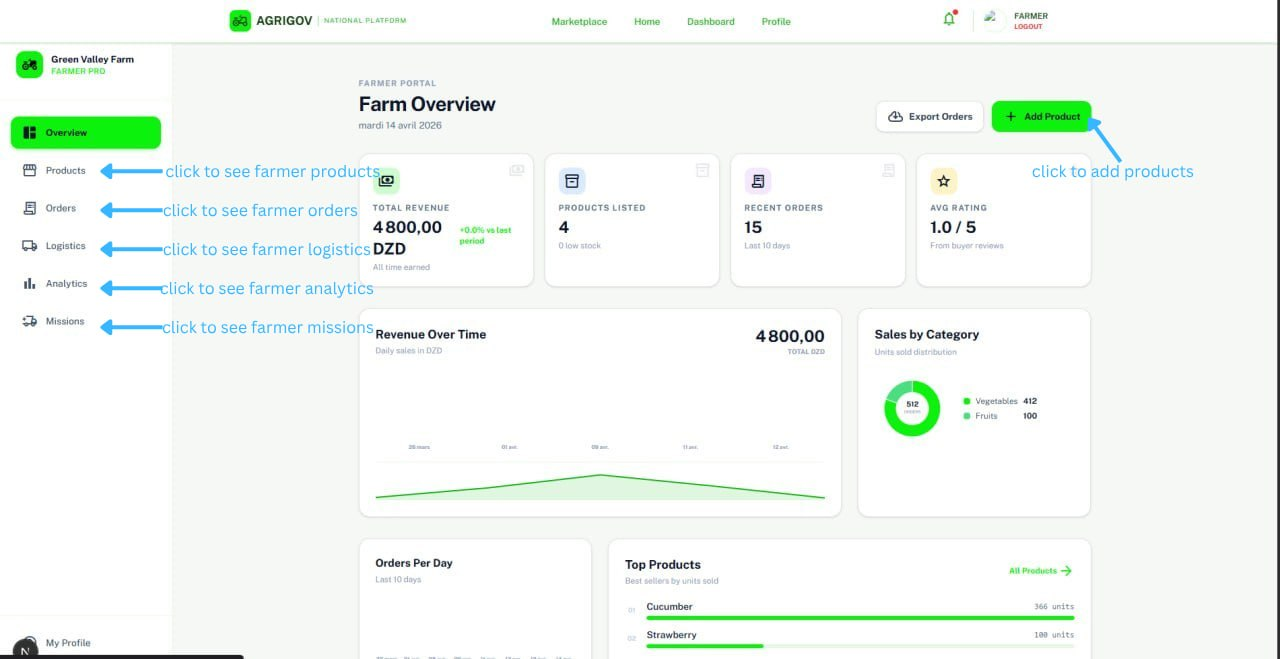
\includegraphics[width=\textwidth]{images/figma/farmer/Overview}
	\caption{Overview Page}
\end{subfigure}
\hfill
\begin{subfigure}[b]{0.45\textwidth}
	\centering
	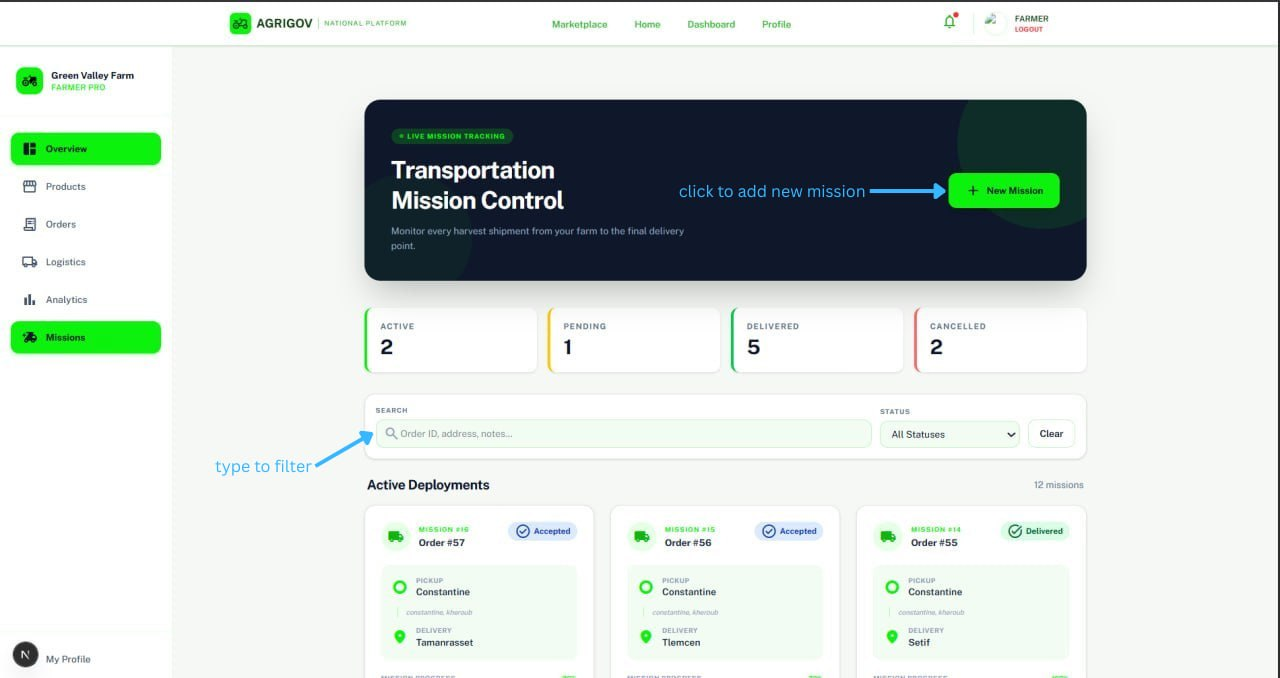
\includegraphics[width=\textwidth]{images/figma/farmer/Transportation mission control}
	\caption{Transportation mission control}
\end{subfigure}

\vspace{0.5cm}
\end{figure}
\begin{figure}[H]
	\centering
	
	% Row 1
	\begin{subfigure}[b]{0.45\textwidth}
		\centering
		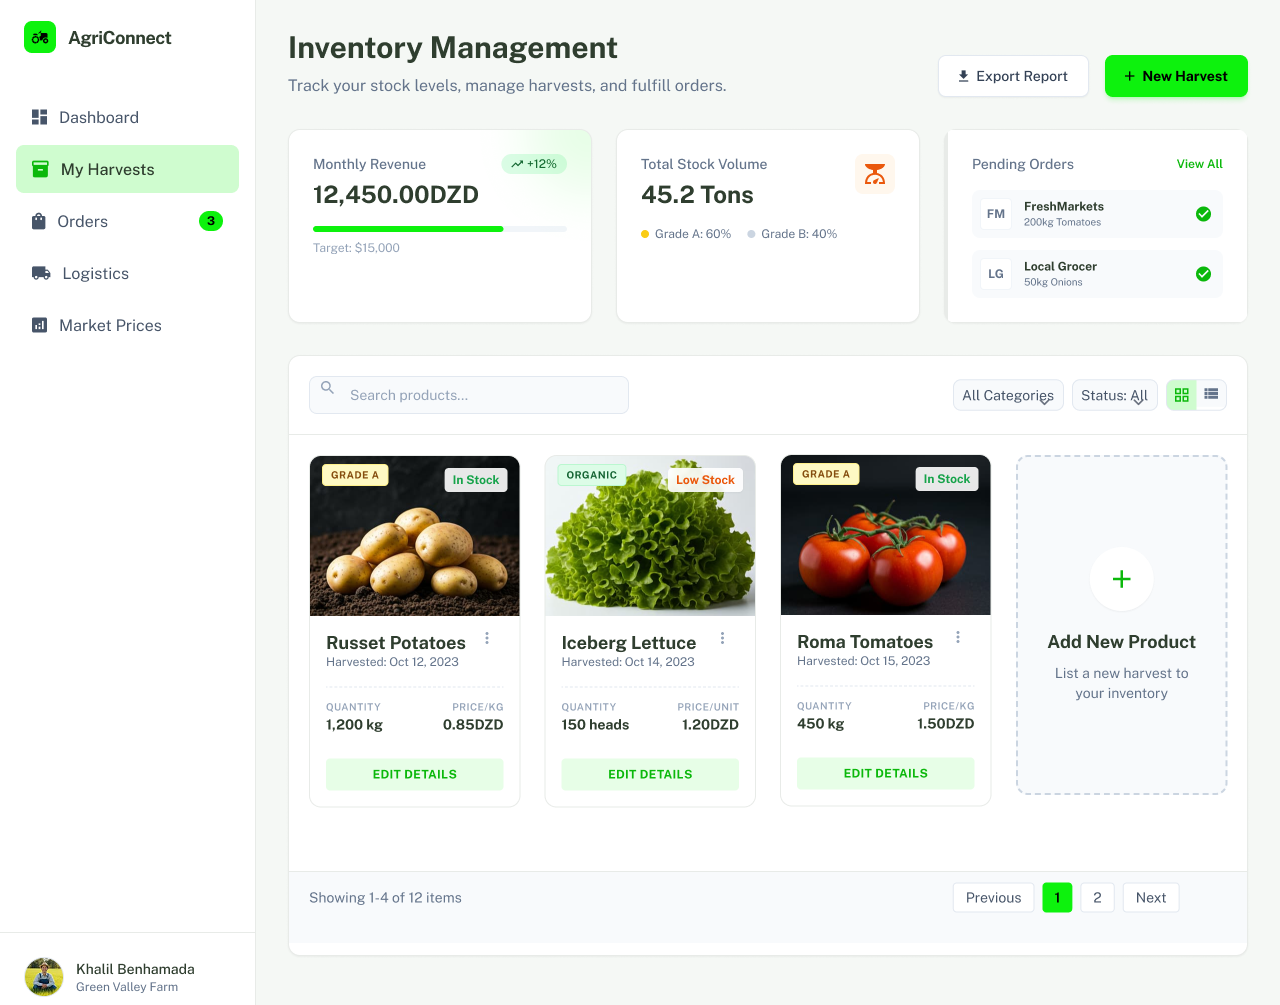
\includegraphics[width=\textwidth]{images/figma/farmer/Farmer Inventory Management}
		\caption{Farmer Inventory Management}
	\end{subfigure}
	\hfill
	\begin{subfigure}[b]{0.45\textwidth}
		\centering
		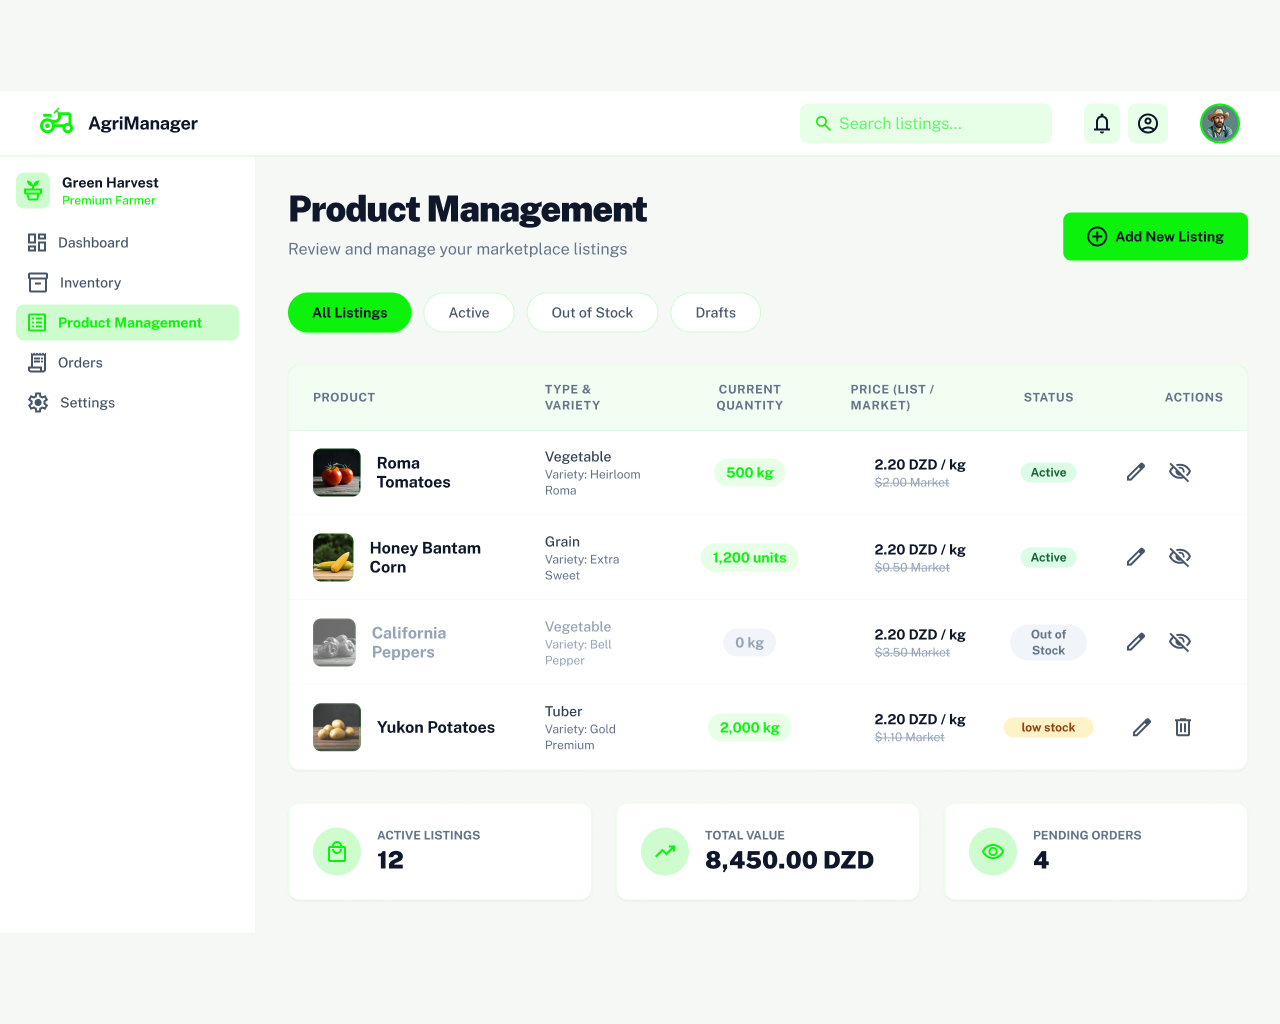
\includegraphics[width=\textwidth]{images/figma/farmer/Product Management}
		\caption{Add New Product}
	\end{subfigure}
	
	\vspace{0.5cm}
	
	% Row 2
	
	\hfill
	
	% Mobile stacked in same column
	\begin{subfigure}[b]{0.95\textwidth}
		\centering
		\begin{subfigure}[b]{0.45\textwidth}
			\centering
			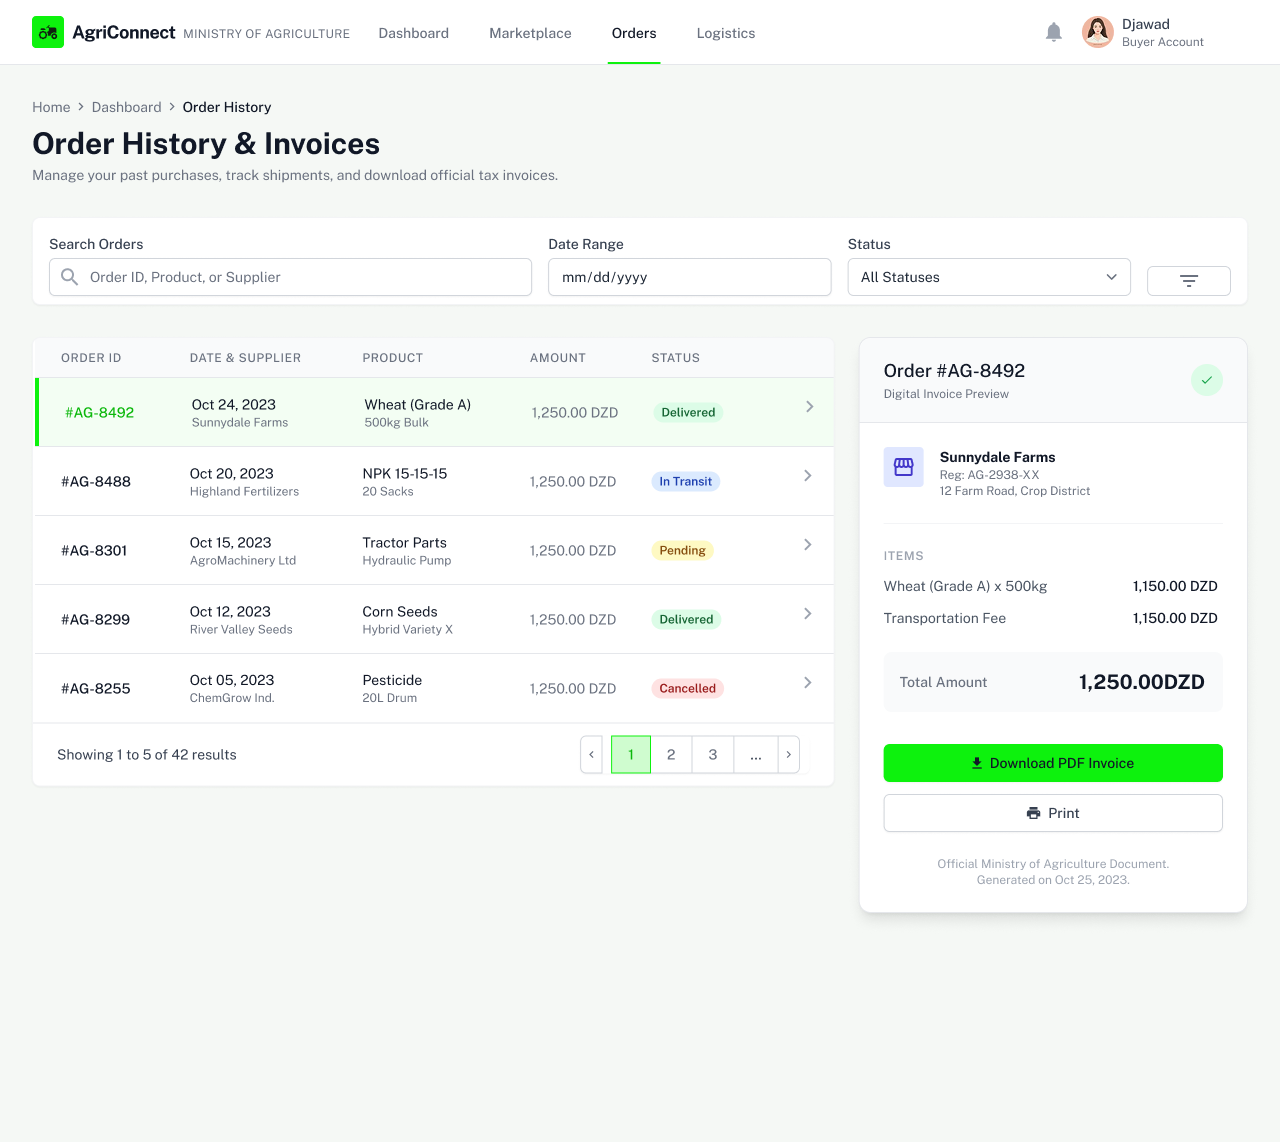
\includegraphics[width=\textwidth]{images/figma/farmer/Order History and Invoices}
			\caption{Order History and Invoices}
		\end{subfigure}
		\hfill
			% Mobile stacked in same column
		\begin{subfigure}[b]{0.17\textwidth}
			\centering
			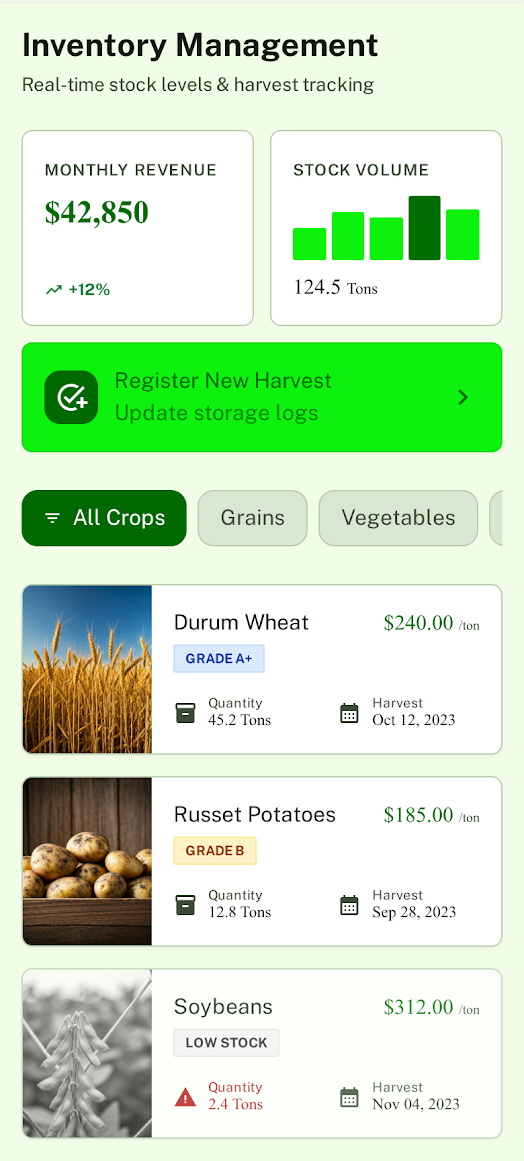
\includegraphics[width=\textwidth]{images/mobile/exports/inventorymanagement}
			\caption{Mobile Login}
		\end{subfigure}
		\hfill
		\begin{subfigure}[b]{0.17\textwidth}
			\centering
			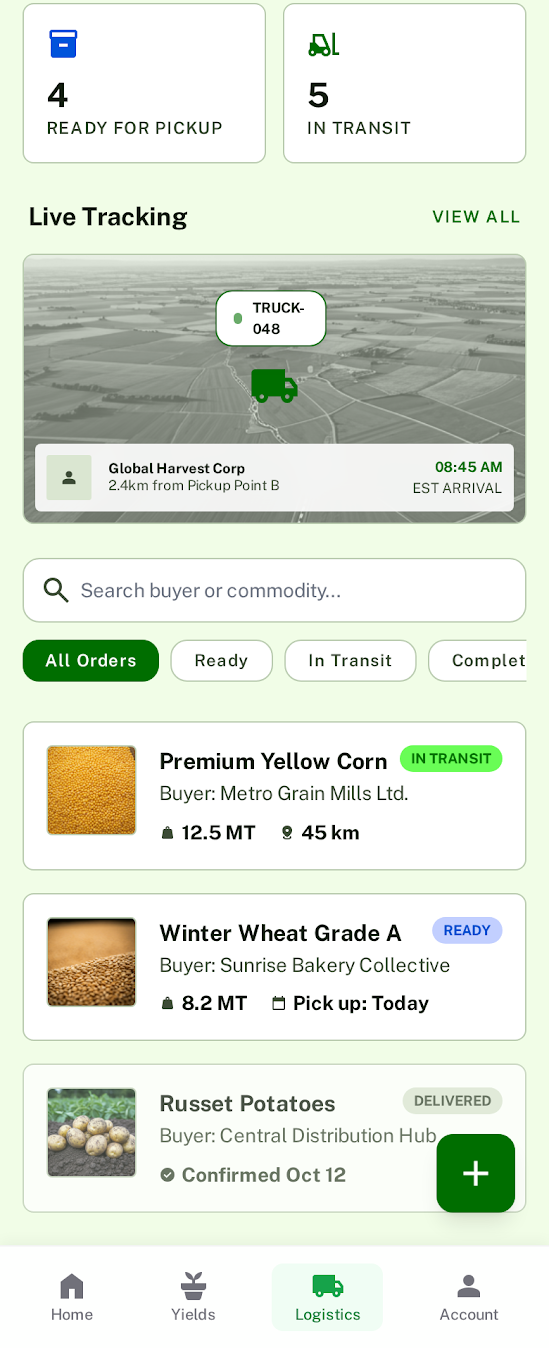
\includegraphics[width=\textwidth]{images/mobile/exports/logistics}
			\caption{Mobile Registration}
		\end{subfigure}
		\hfill
		\begin{subfigure}[b]{0.17\textwidth}
			\centering
			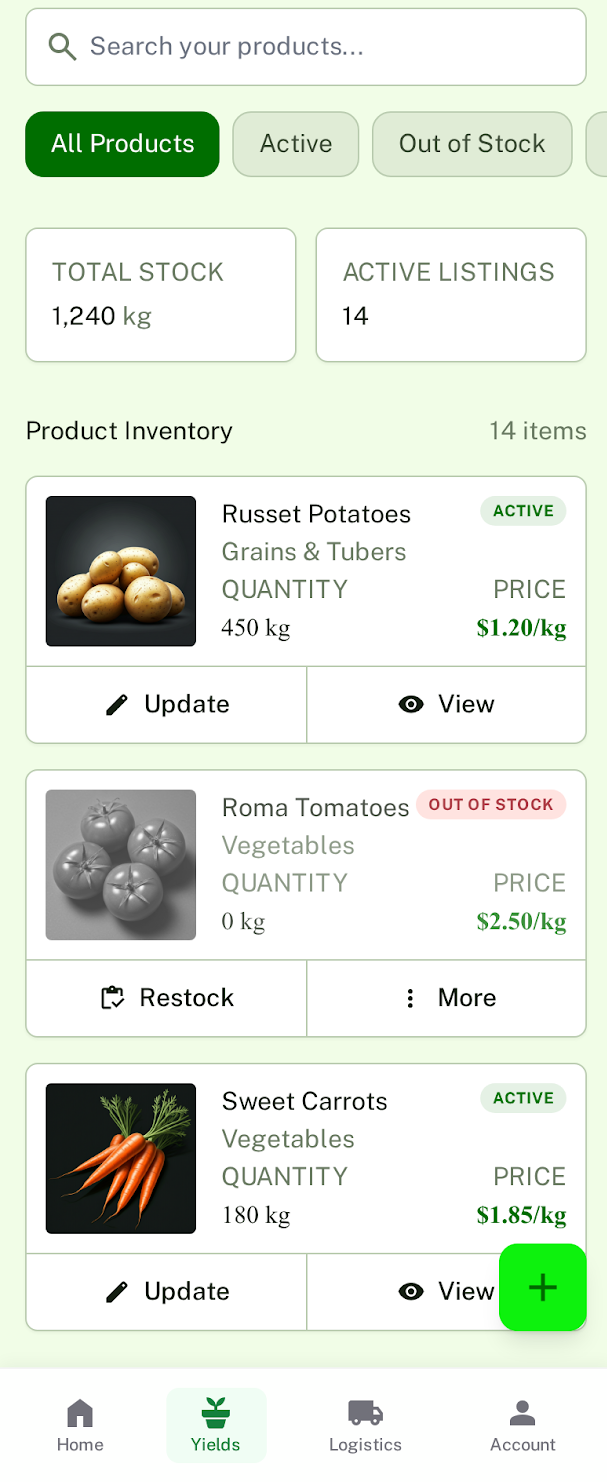
\includegraphics[width=\textwidth]{images/mobile/exports/productManagement}
			\caption{Mobile Registration}
		\end{subfigure}
		
	\end{subfigure}
	
	\caption{Farmer Interface Mockups}
	\label{fig:farmer-ui}
\end{figure}

%----------------------------------------------------
\subsection{Buyer Interface}
\begin{figure}[H]
	\centering
	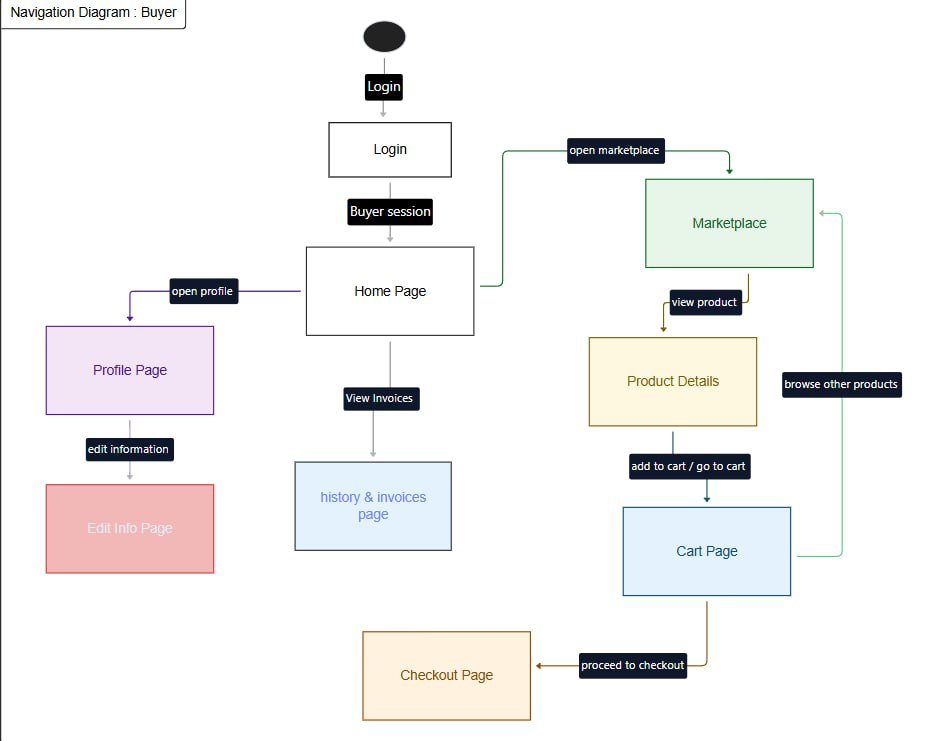
\includegraphics[width=0.9\textwidth]{images/navigation/buyer-navigation}
	\caption{Buyer Navigation Diagram}
	\label{fig:buyer-navigation}
\end{figure}
\begin{figure}[H]
	\centering
	\begin{subfigure}[b]{0.45\textwidth}
		\centering
		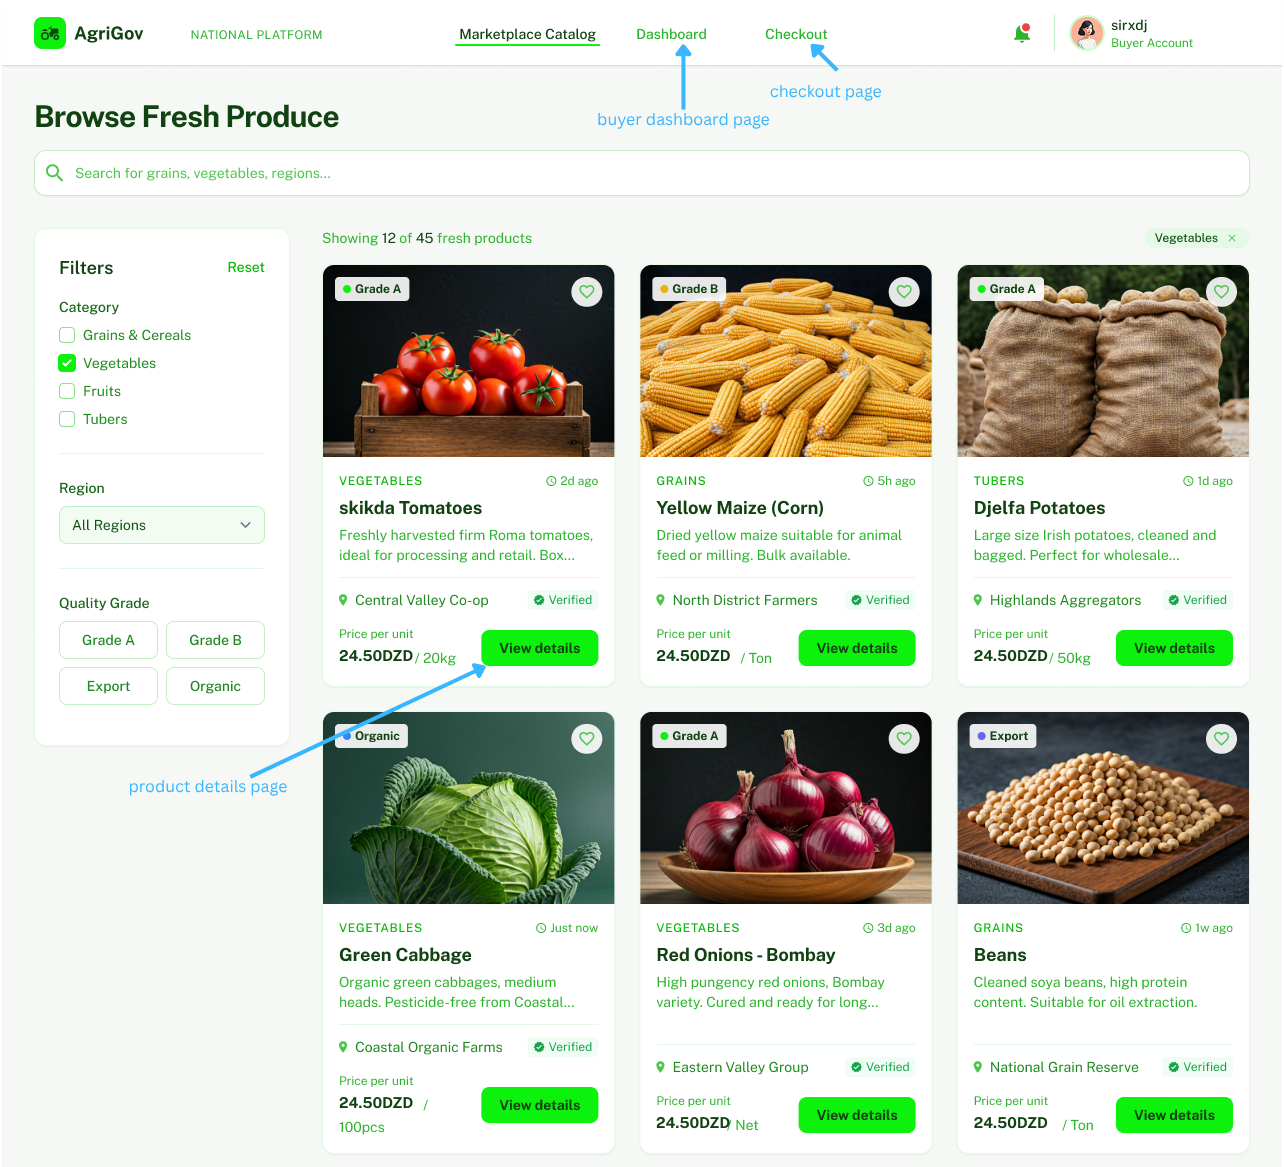
\includegraphics[width=\textwidth]{images/figma/buyer/Buyer Marketplace Catalog}
		\caption{Marketplace Product Catalog}
	\end{subfigure}
	\hfill
	\begin{subfigure}[b]{0.45\textwidth}
		\centering
		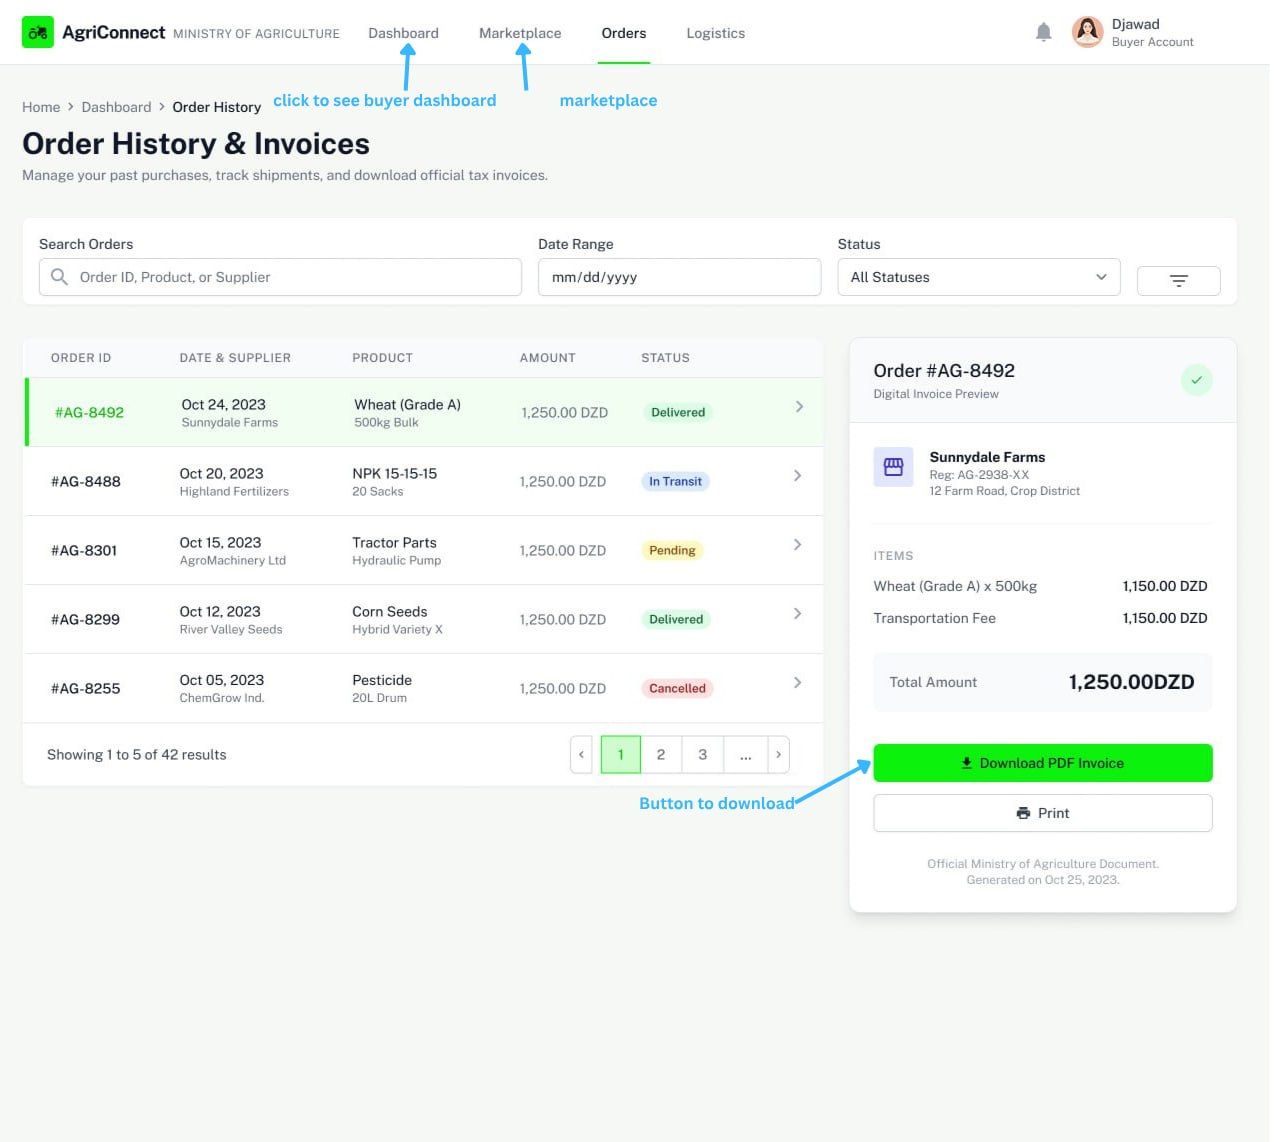
\includegraphics[width=\textwidth]{images/figma/buyer/order history}
		\caption{Buyer Order History}
	\end{subfigure}
	
	\vspace{0.5cm}
\end{figure}
\begin{figure}[H]
	\centering
	
	
	
	\begin{subfigure}[b]{0.45\textwidth}
		\centering
		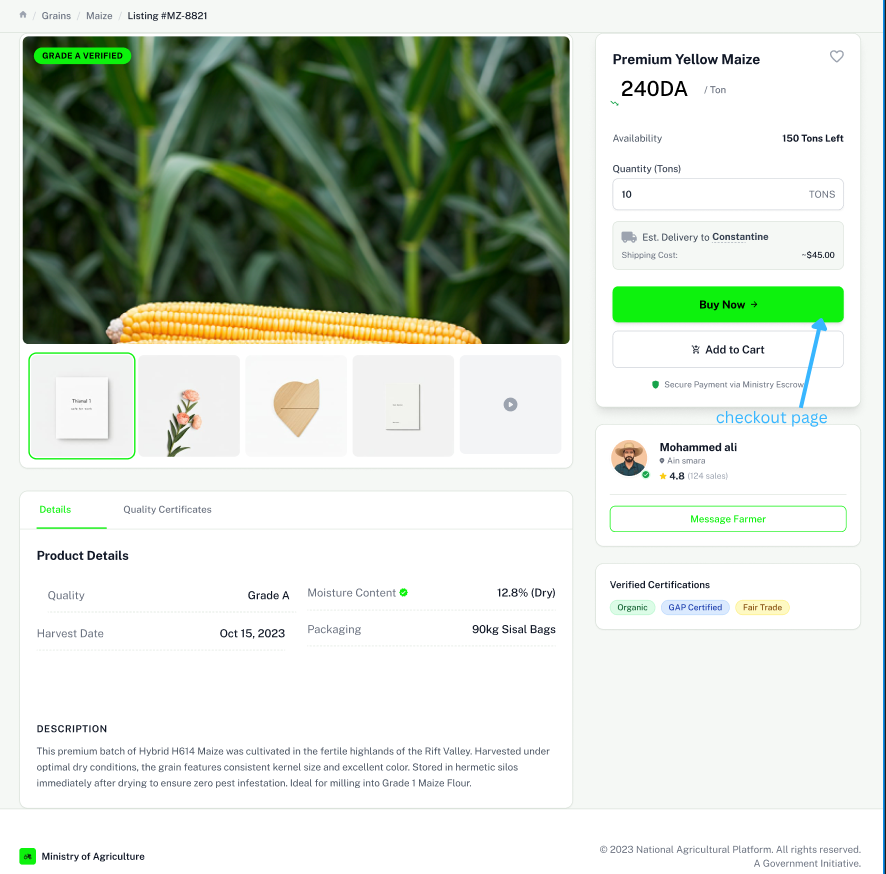
\includegraphics[width=\textwidth]{images/figma/buyer/Product Specification Details}
		\caption{Product Specification Details}
	\end{subfigure}
	\hfill
	\begin{subfigure}[b]{0.17\textwidth}
		\centering
		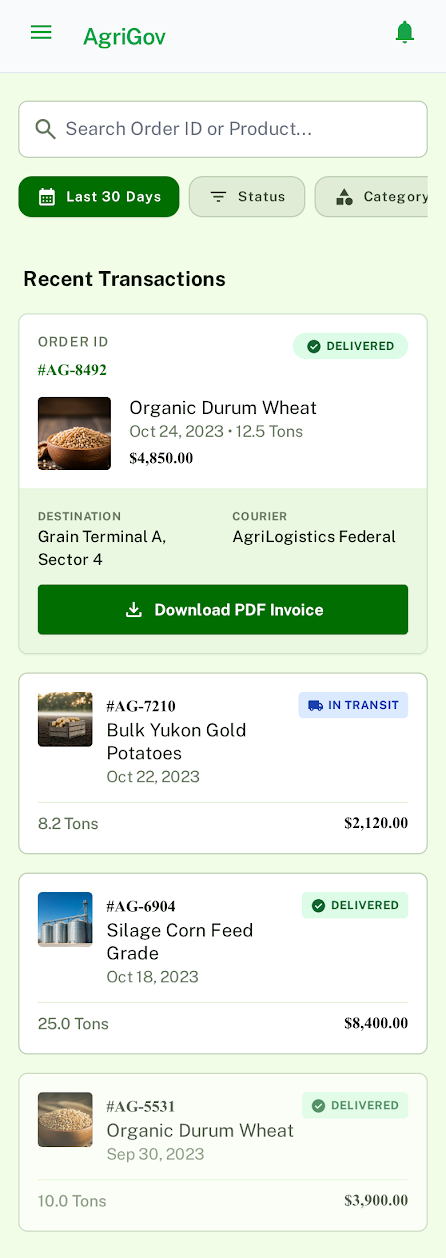
\includegraphics[width=\textwidth]{images/mobile/exports/orderhistory}
		\caption{Order History mobile}
	\end{subfigure}
	\begin{subfigure}[b]{0.17\textwidth}
		\centering
		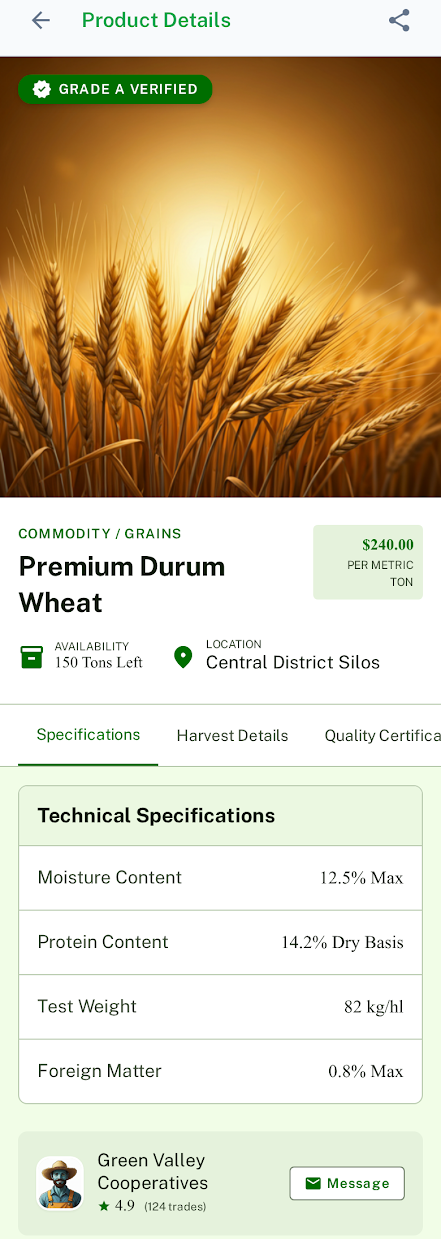
\includegraphics[width=\textwidth]{images/mobile/exports/productdetail}
		\caption{Product detail mobile}
	\end{subfigure}
	\begin{subfigure}[b]{0.17\textwidth}
		\centering
		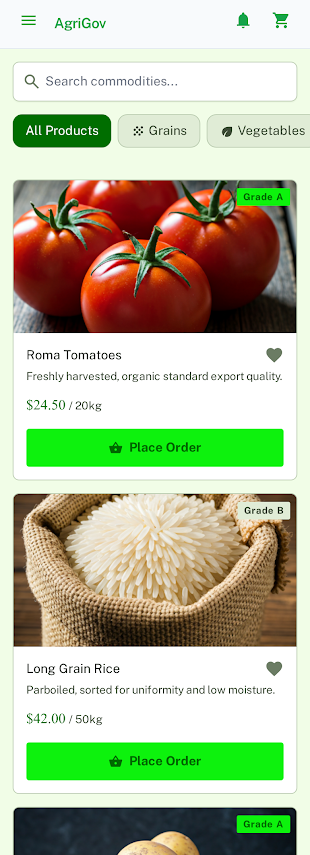
\includegraphics[width=\textwidth]{images/mobile/exports/catalog}
		\caption{Catalogue mobile}
	\end{subfigure}
	
	\caption{Buyer Interface Mockups}
	\label{fig:buyer-ui}
	
\end{figure}

%----------------------------------------------------
\subsection{Transporter Interface}
\begin{figure}[H]
	\centering
	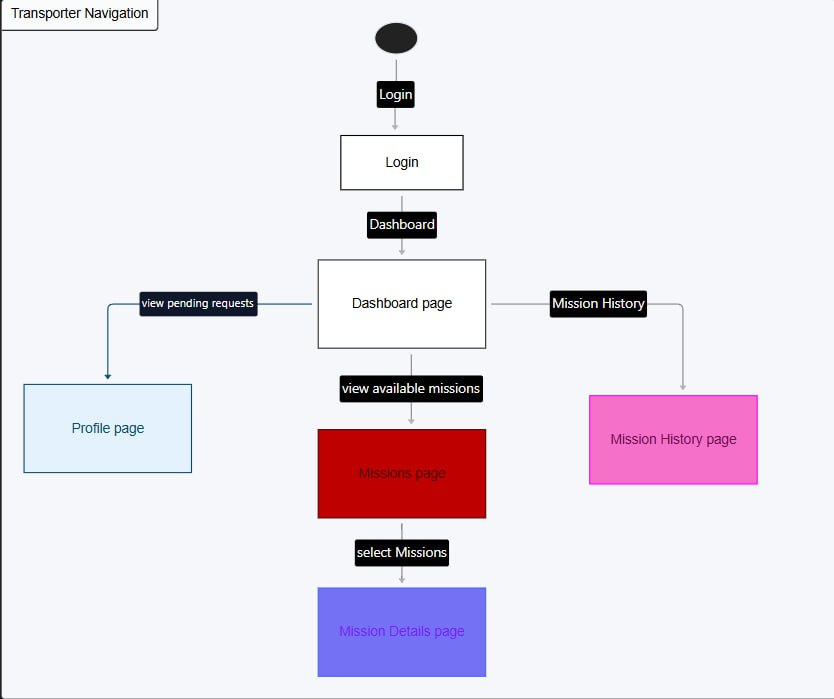
\includegraphics[width=0.9\textwidth]{images/navigation/transporter-navigation}
	\caption{Transporter Navigation Diagram}
	\label{fig:transporter-navigation}
\end{figure}
\begin{figure}[H]
	\centering
	
	\begin{subfigure}[b]{0.45\textwidth}
		\centering
		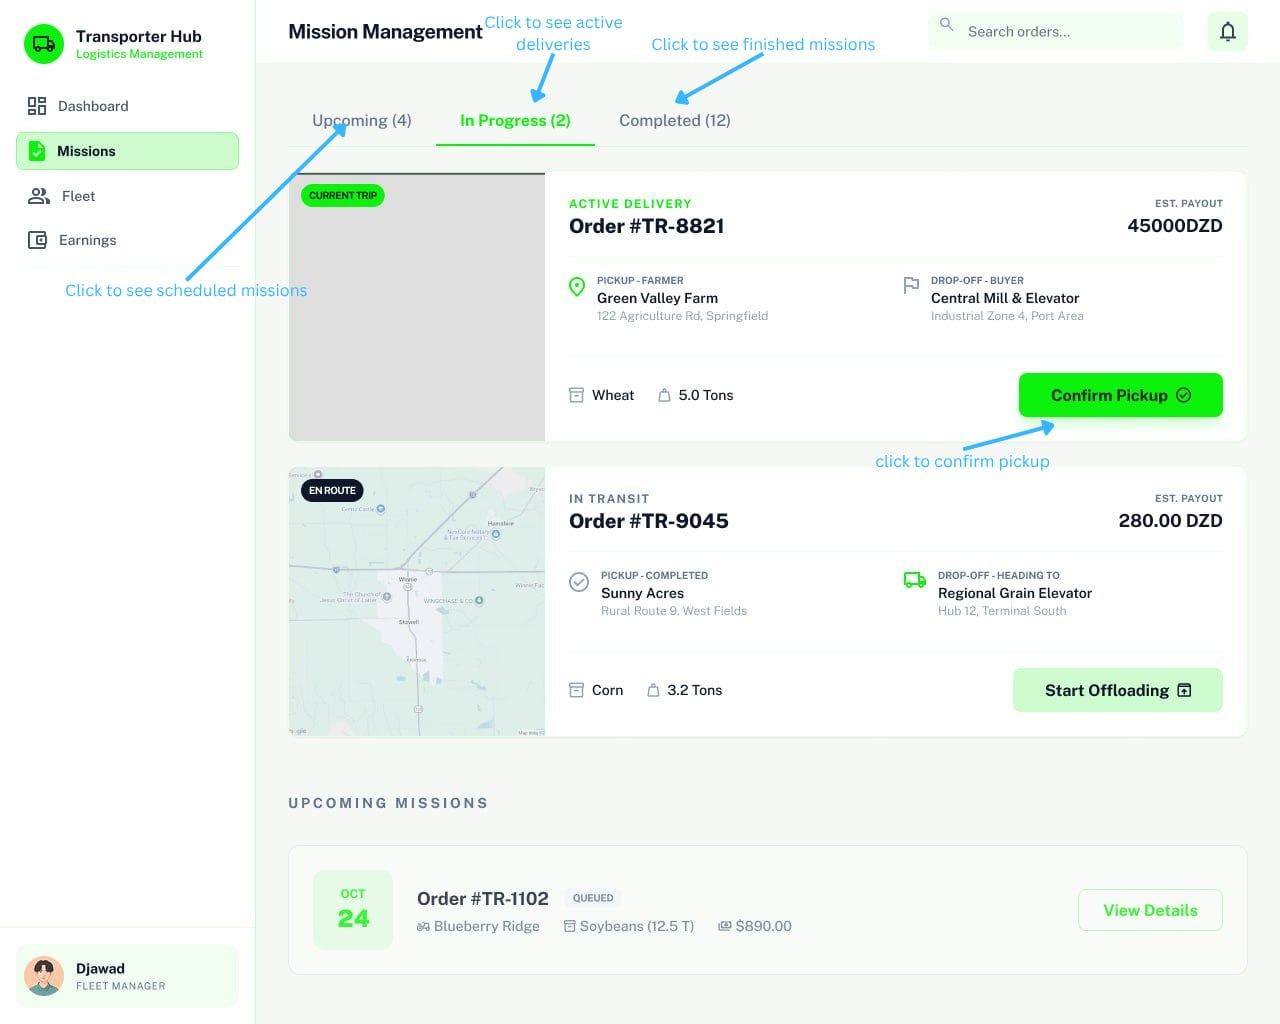
\includegraphics[width=\textwidth]{images/figma/transporter/Body-1}
		\caption{Transporter Dashboard}
	\end{subfigure}
	\hfill
	\begin{subfigure}[b]{0.45\textwidth}
		\centering
		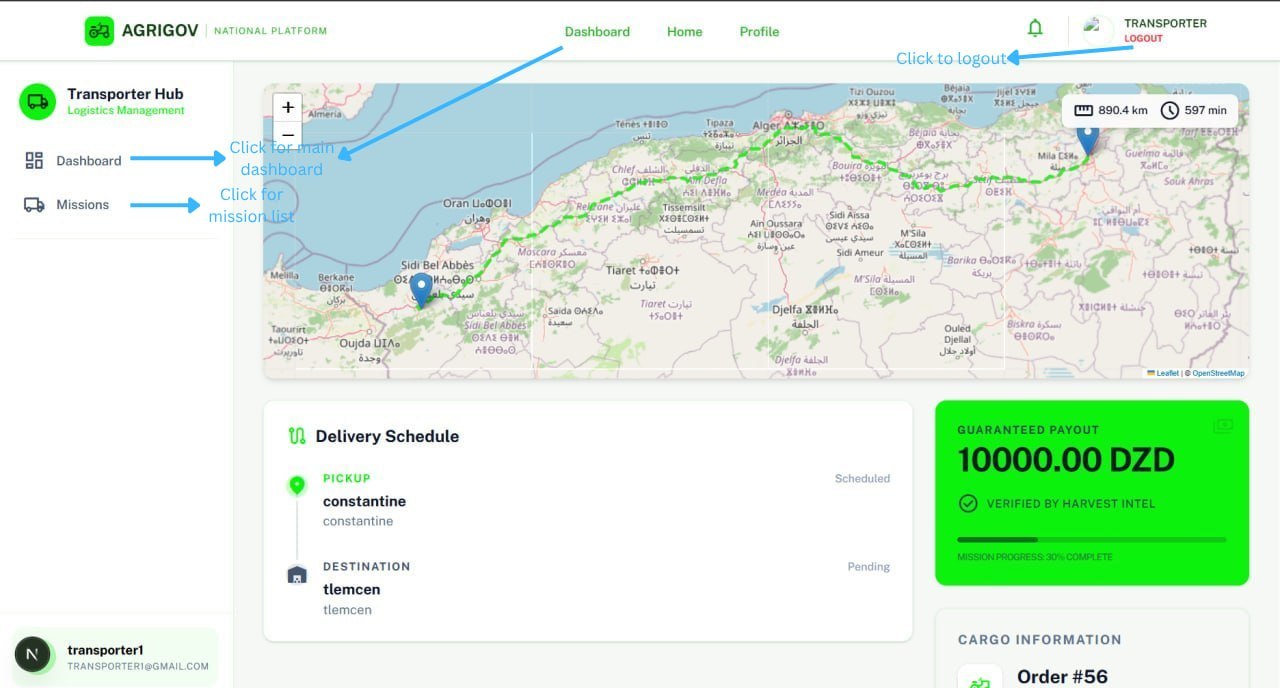
\includegraphics[width=\textwidth]{images/figma/transporter/Transporter Mission Control}
		\caption{Transporter Mission Control}
	\end{subfigure}
	
	
	
	
\end{figure}
\begin{figure}[H]
	\centering
	
	
	
	\begin{subfigure}[b]{0.17\textwidth}
		\centering
		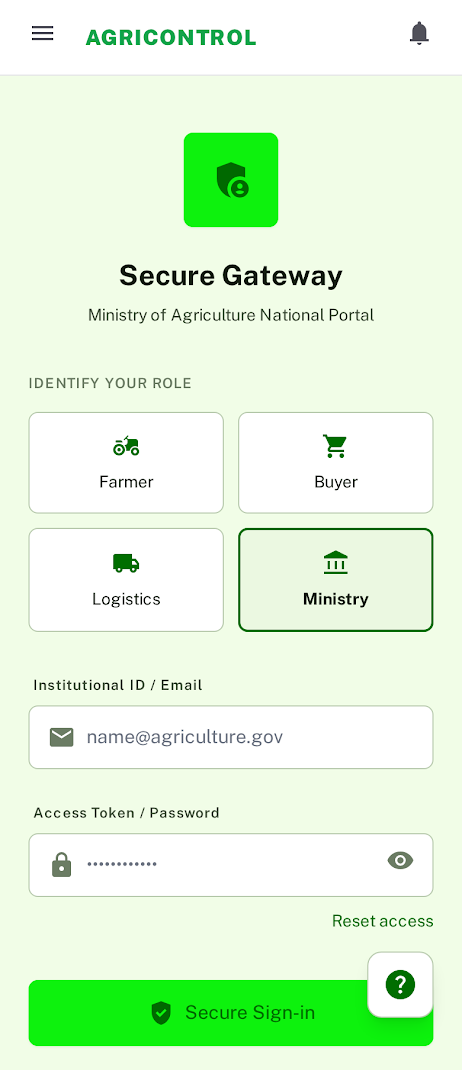
\includegraphics[width=\textwidth]{images/mobile/exports/login}
		\caption{mobile login}
	\end{subfigure}
	\hfill
	\begin{subfigure}[b]{0.17\textwidth}
		\centering
		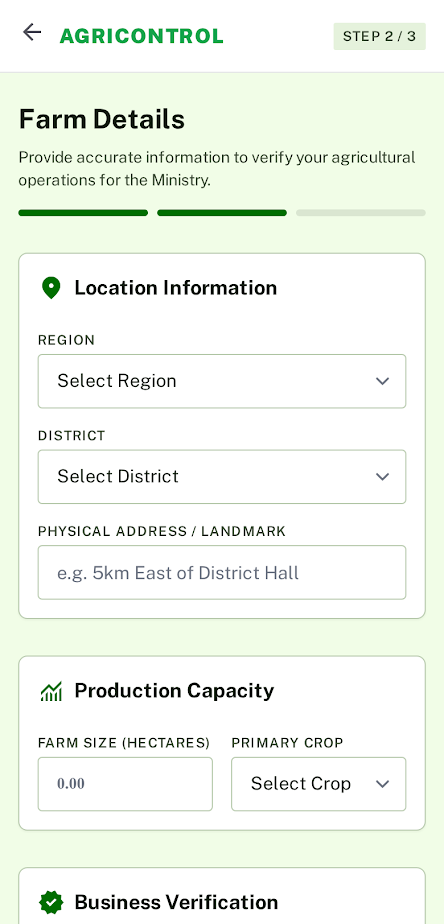
\includegraphics[width=\textwidth]{images/mobile/exports/registration}
		\caption{registration mobile}
	\end{subfigure}
		\hfill
	\begin{subfigure}[b]{0.17\textwidth}
		\centering
		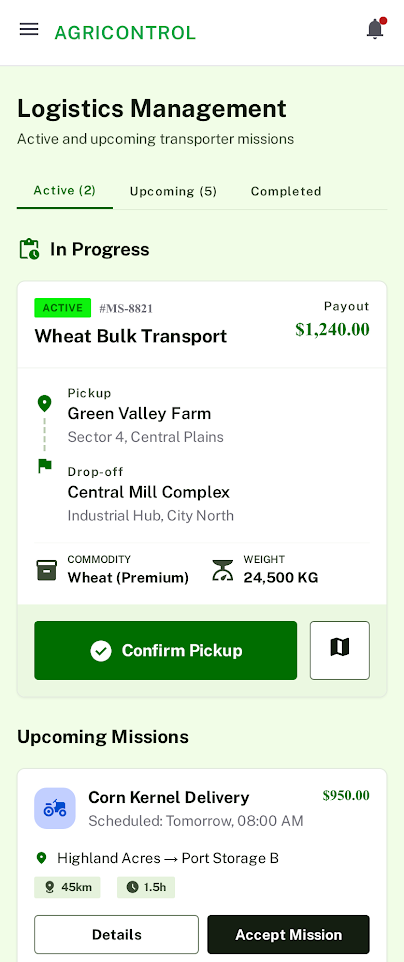
\includegraphics[width=\textwidth]{images/mobile/exports/missions}
		\caption{missions mobile}
	\end{subfigure}
		\hfill
	\begin{subfigure}[b]{0.17\textwidth}
		\centering
		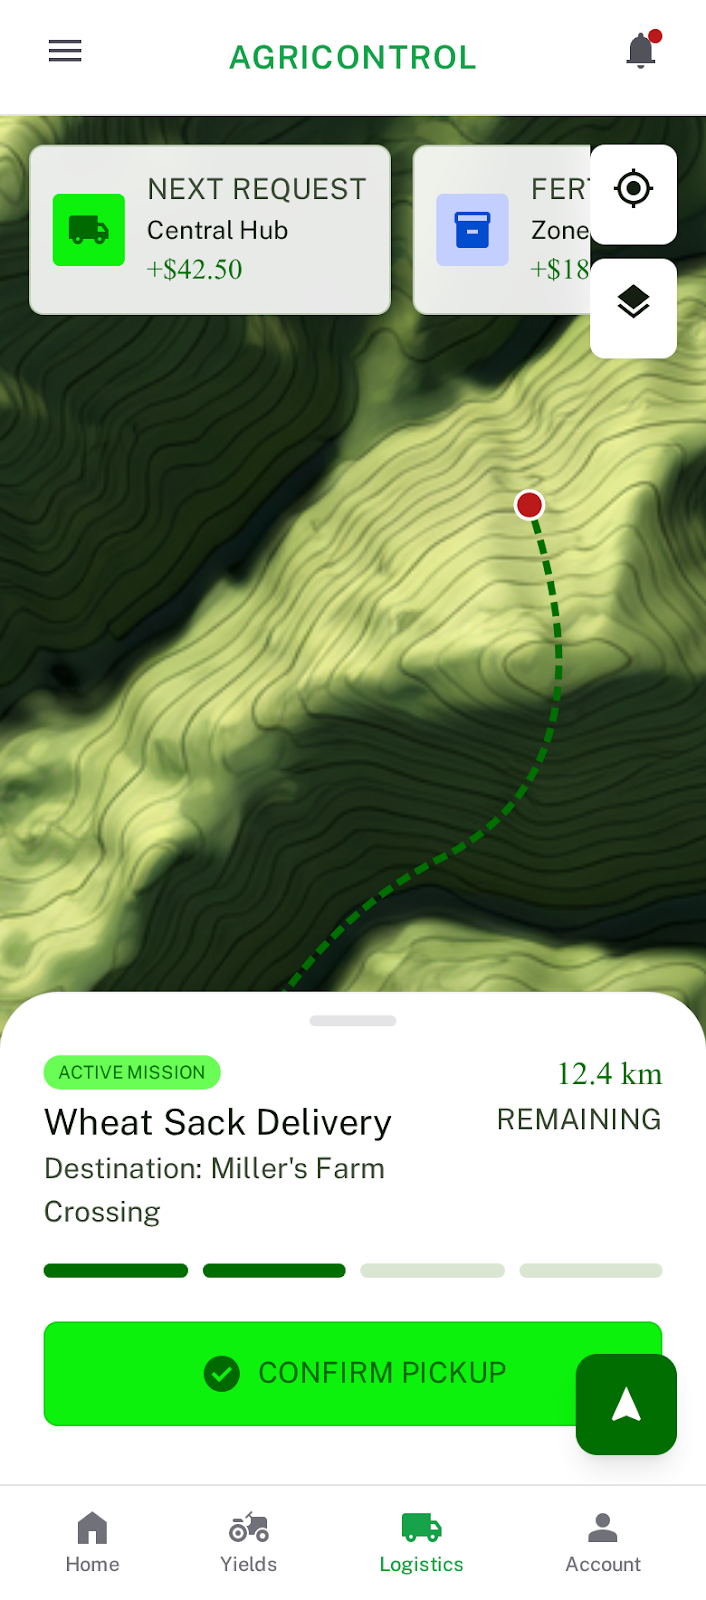
\includegraphics[width=\textwidth]{images/mobile/exports/missioncontrol}
		\caption{mission Controle mobile}
	\end{subfigure}
	
	\caption{Transporter Interface Mockups}
	\label{fig:transporter-ui}
	
\end{figure}

%----------------------------------------------------
\subsection{Ministry Interface}
\begin{figure}[H]
	\centering
	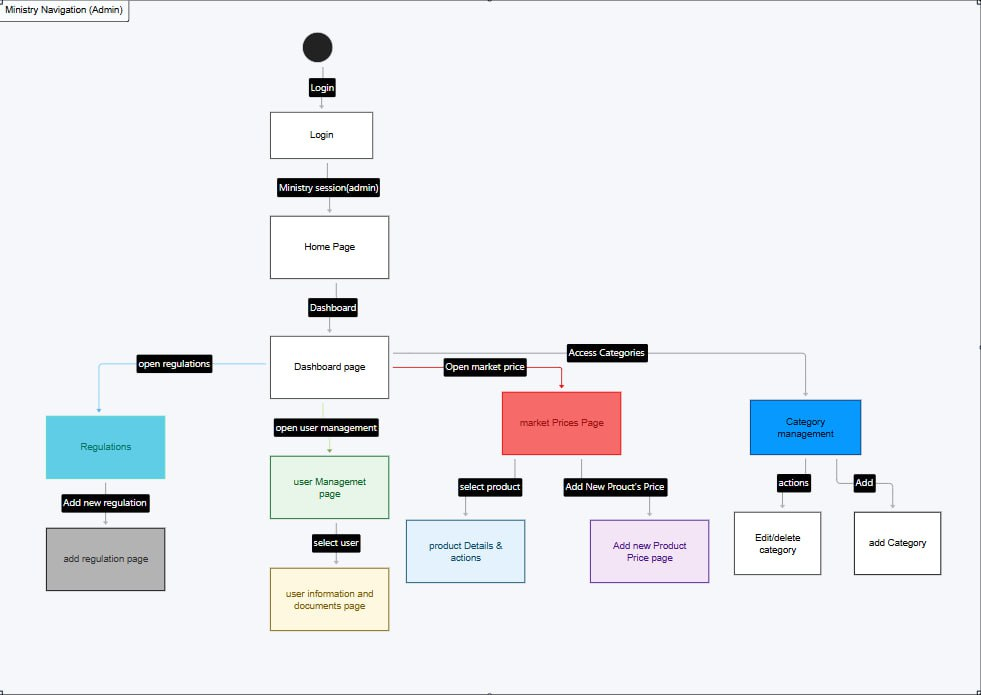
\includegraphics[width=0.9\textwidth]{images/navigation/ministry-navigation}
	\caption{Ministry Navigation Diagram}
	\label{fig:ministry-navigation}
\end{figure}
\begin{figure}[H]
		\centering
	
	\begin{subfigure}[b]{0.45\textwidth}
		\centering
		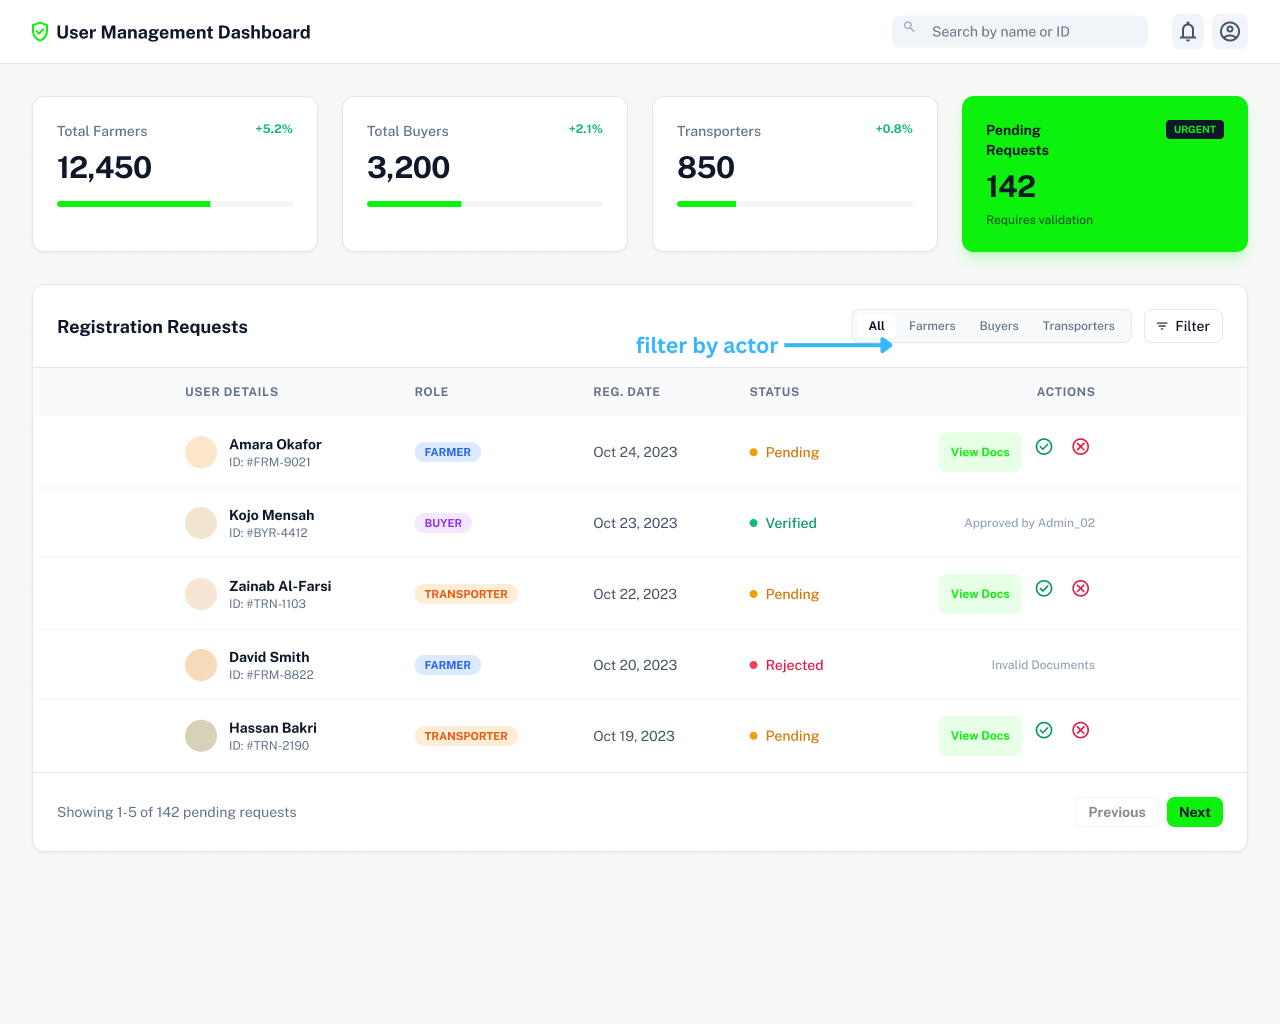
\includegraphics[width=\textwidth]{images/figma/ministry/user management}
		\caption{User Validation Panel}
	\end{subfigure}
	\hfill
	\begin{subfigure}[b]{0.45\textwidth}
		\centering
		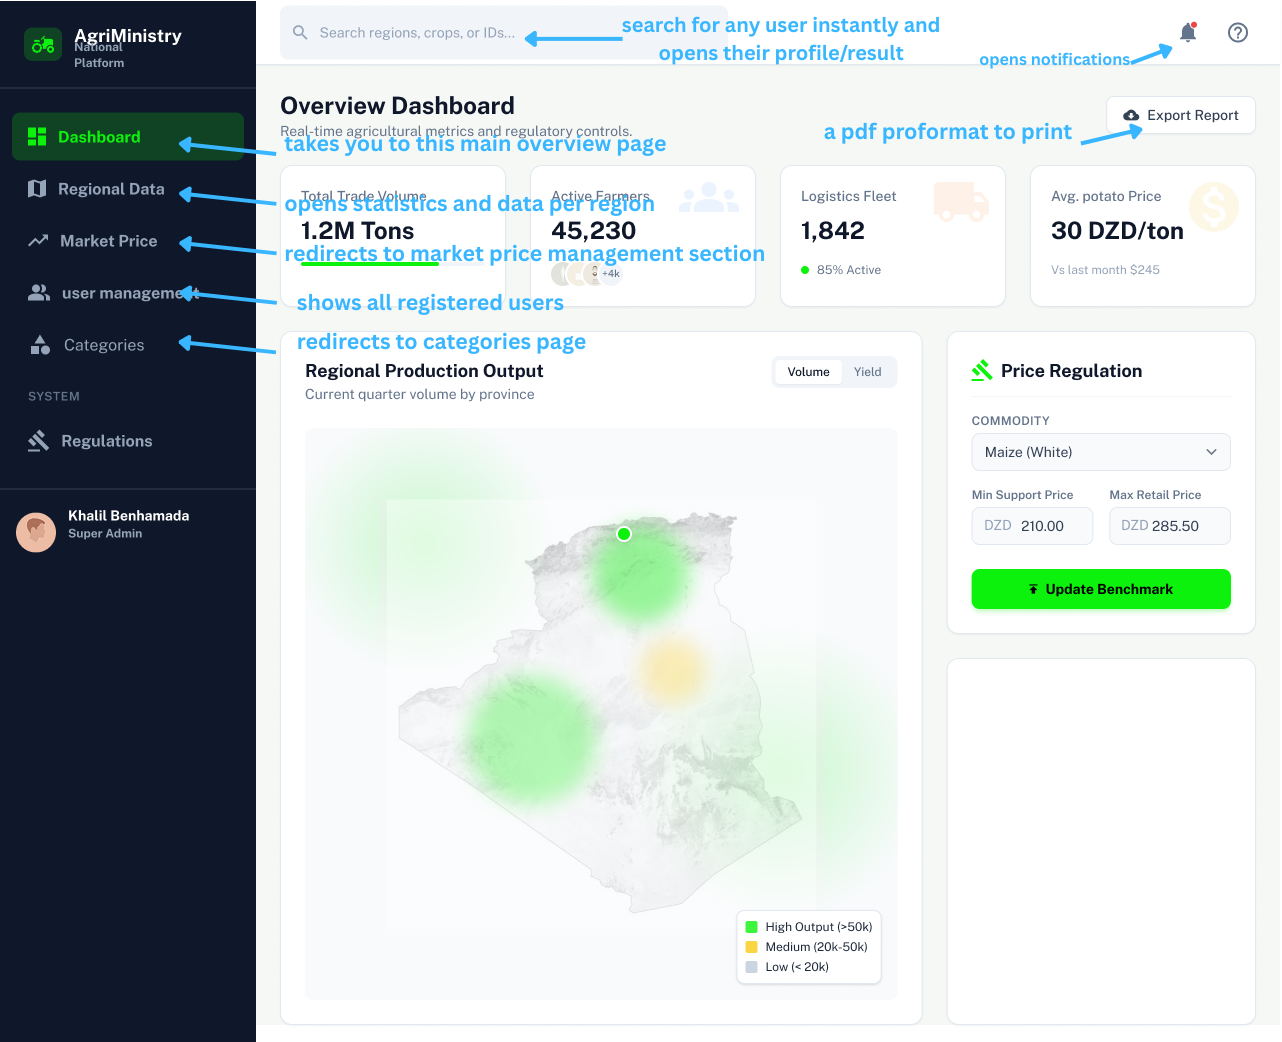
\includegraphics[width=\textwidth]{images/figma/ministry/Ministry Admin Dashboard}
		\caption{Ministry Administration Dashboard}
	\end{subfigure}
	
	\vspace{0.5cm}
\end{figure}
\begin{figure}[H]
	\centering
	
	\begin{subfigure}[b]{0.45\textwidth}
		\centering
		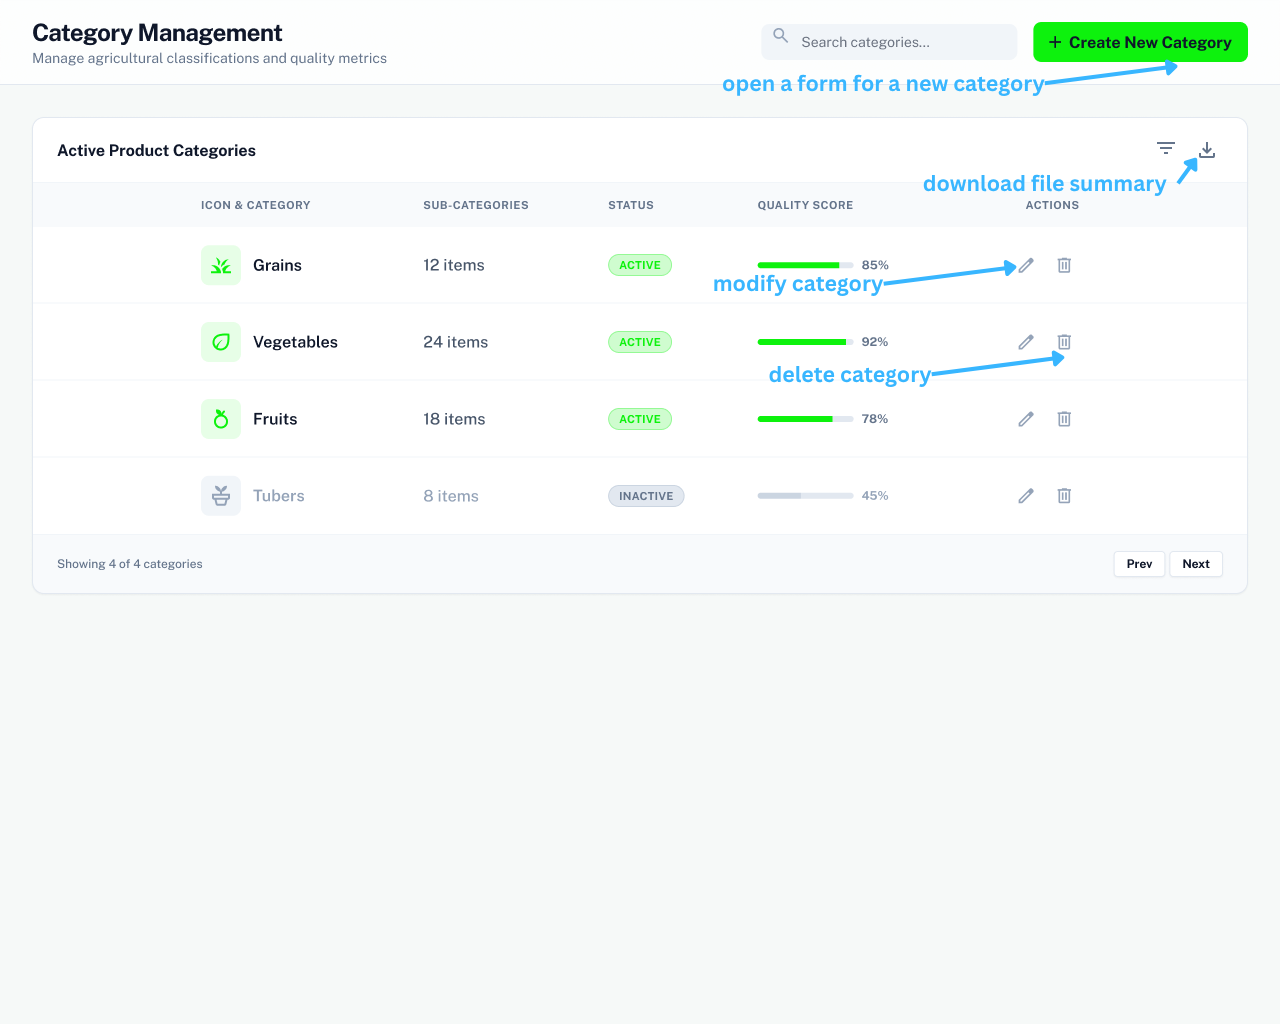
\includegraphics[width=\textwidth]{images/figma/ministry/category}
		\caption{Category management}
	\end{subfigure}
	\hfill
	\begin{subfigure}[b]{0.45\textwidth}
		\centering
		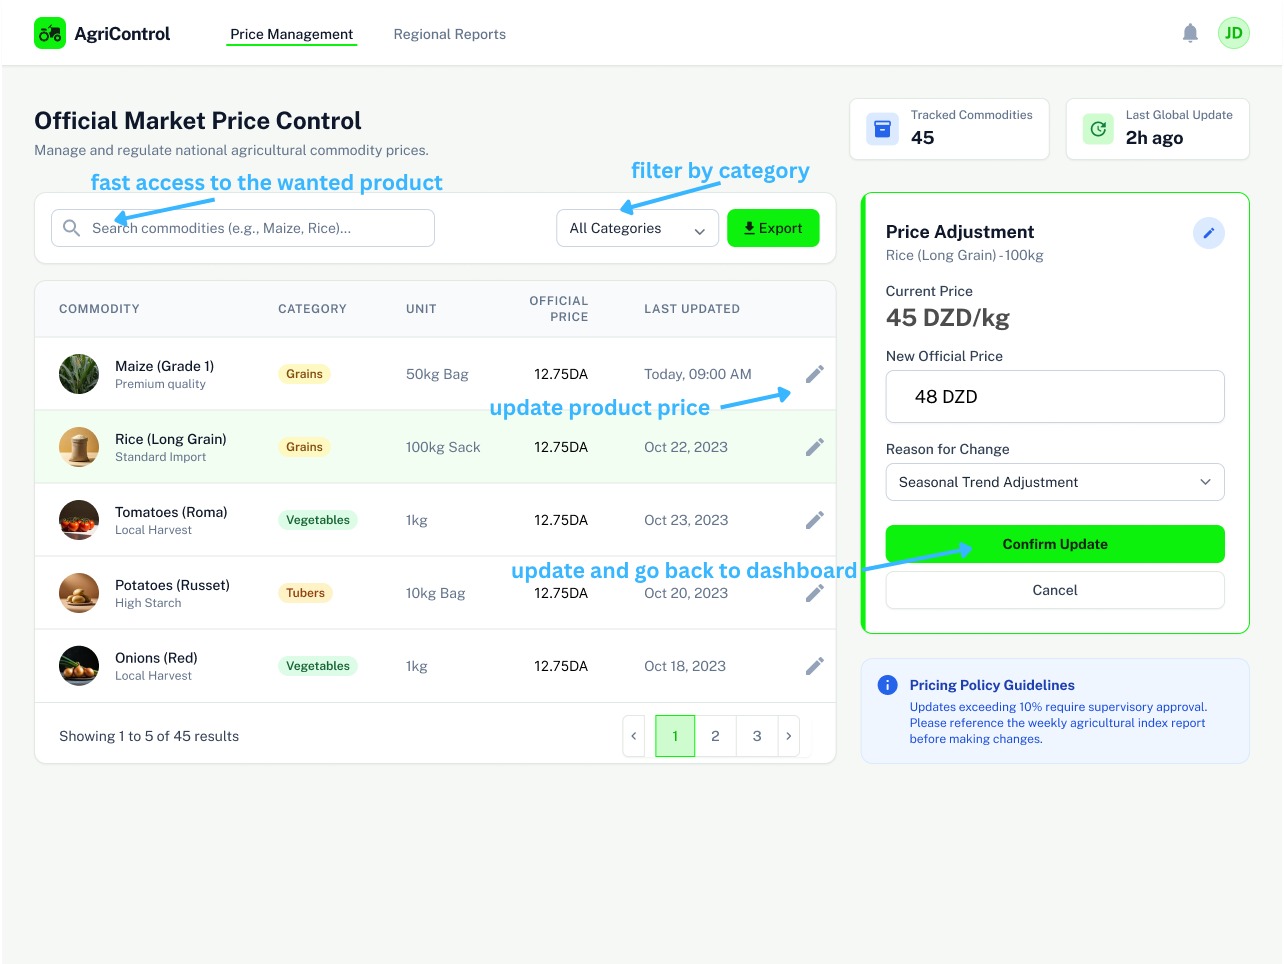
\includegraphics[width=\textwidth]{images/figma/ministry/Official Price Management}
		\caption{Official Price Management}
	\end{subfigure}
	
	\caption{Ministry Interface Mockups}
	\label{fig:ministry-ui}
	
\end{figure}

% 7) Conclusion
\section{Conclusion}

The analysis phase presented in this chapter provides a clear and comprehensive understanding of the functional and technical requirements for the \textbf{AgriGov Market} platform. By examining the current limitations of the Algerian agricultural market—specifically the issues of informal intermediation and price opacity—we have established a robust foundation for a digital intervention. Through the identification of key actors and the modeling of use cases, we have defined the essential interactions required to connect farmers, buyers, and transporters within a regulated environment supervised by the Ministry of Agriculture.

The detailed textual descriptions and system sequence diagrams developed in this chapter serve as a formal specification that ensures the system addresses the real-world needs of its users. This requirements gathering process has successfully translated the project’s strategic objectives into a set of well-defined functionalities, including product management, transparent order processing, and logistics coordination. With these functional boundaries and user expectations now clearly established, the project is ready to move from the analytical phase to the architectural phase. In the following chapter, we will focus on the system design, where these requirements will be transformed into a technical blueprint, covering the structural modeling, database schema, and the physical architecture of the application.